% ============================================================================
% FL-EHDS Paper for FLICS 2026 — Condensed 8-page version
% IEEE Conference Format (max 8 pages including references)
% February 2026
% ============================================================================

\documentclass[conference,a4paper]{IEEEtran}

% ===== PACKAGES =====
\usepackage{cite}
\usepackage{amsmath,amssymb,amsfonts}
\usepackage{graphicx}
\usepackage{textcomp}
\usepackage{xcolor}
\usepackage{booktabs}
\usepackage{hyperref}
\usepackage{url}

% TikZ for vector figures
\usepackage{tikz}
\usetikzlibrary{shapes.geometric, arrows.meta, positioning, fit, backgrounds, calc}
\usepackage{pgfplots}
\pgfplotsset{compat=1.18}

% ===== DOCUMENT =====
\begin{document}

\title{FL-EHDS: A Privacy-Preserving Federated Learning Framework for the European Health Data Space}

\author{
    \IEEEauthorblockN{Fabio Liberti}
    \IEEEauthorblockA{
        Department of Computer Science\\
        Universitas Mercatorum, Rome, Italy\\
        fabio.liberti@unimercatorum.it\\
        ORCID: 0000-0003-3019-5411
    }
}

\maketitle

% ============================================================================
% ABSTRACT
% ============================================================================
\begin{abstract}
The European Health Data Space (EHDS), established by Regulation (EU) 2025/327, mandates cross-border health data analytics while preserving citizen privacy. Federated Learning (FL) is the key enabling technology for secondary use, yet only 23\% of FL implementations achieve sustained production deployment in healthcare. We present FL-EHDS, a three-layer compliance framework integrating governance mechanisms (Health Data Access Bodies, data permits, opt-out registries), FL orchestration (17 aggregation algorithms including 2024--2025 advances, differential privacy, secure aggregation), and data holder components (adaptive training, FHIR preprocessing). Experimental validation on 5 tabular clinical datasets---including the European-origin PTB-XL ECG with natural 52-site partitioning---with 3 additional imaging datasets under evaluation, demonstrates that personalized FL (Ditto) narrows the centralized-federated gap to 6.6 percentage points while preserving full data sovereignty, and that algorithm choice produces up to 18.7pp accuracy differences on heterogeneous clinical data. Our systematic evidence synthesis of 47 documents reveals that legal uncertainties---not technical barriers---constitute the critical blocker for FL adoption in EHDS contexts. The open-source reference implementation and compliance mapping provide actionable guidance for the 2025--2031 transition period.
\end{abstract}

\begin{IEEEkeywords}
Federated Learning, European Health Data Space, Privacy-Preserving Technologies, GDPR, Health Data Governance, Cross-Border Analytics
\end{IEEEkeywords}

% ============================================================================
% 1. INTRODUCTION
% ============================================================================
\section{Introduction}
\label{sec:introduction}

The European Health Data Space (EHDS), established by Regulation (EU) 2025/327, represents the EU's most ambitious initiative for cross-border health data governance~\cite{eu2025ehds}. Entering into force in March 2025, the regulation creates a dual framework: primary use through MyHealth@EU for patient care, and secondary use through HealthData@EU for research, innovation, and policy-making~\cite{ganna2024boost}. Health Data Access Bodies (HDABs) in each Member State authorize secondary use through data permits; Article~53 enumerates permitted purposes; Article~71 introduces citizen opt-out mechanisms~\cite{staunton2024ethical}. The implementation timeline extends to 2031, with delegated acts expected by March 2027 and secondary use provisions applicable from March 2029.

Federated Learning (FL) emerges as the ideal technical solution for EHDS secondary use---the model travels to distributed data rather than centralizing sensitive records~\cite{mcmahan2017communication, kairouz2021advances, rieke2020future}. The COVID-19 pandemic demonstrated FL's potential at scale: Dayan et al.~\cite{dayan2021federated} trained a global model across 20 institutions in 5 countries. However, recent evidence reveals a sobering gap between FL's promise and operational reality. Fr\"ohlich et al.~\cite{frohlich2025reality} report that only 23\% of FL implementations achieve sustained production deployment, with hardware heterogeneity (78\%) and non-IID data distributions (67\%) as dominant barriers. Beyond technical constraints, legal uncertainties regarding gradient data status under GDPR remain unresolved~\cite{quinn2024gdpr}, while van Drumpt et al.~\cite{vandrumpt2025pets} demonstrate that privacy-enhancing technologies cannot substitute for robust governance frameworks.

Prior FL frameworks for healthcare~\cite{rieke2020future, sheller2020federated} focus on technical architectures without addressing regulatory compliance. Legal analyses~\cite{quinn2024gdpr, staunton2024ethical, shabani2024ehds} examine GDPR constraints but abstract from implementation feasibility. Policy documents~\cite{tehdas2024ready} assess Member State readiness but do not integrate FL technical considerations. To our knowledge, no existing work provides an integrated framework addressing all three dimensions: systematic barrier evidence, technical implementation with state-of-the-art algorithms, and EHDS governance operationalization---a gap confirmed by recent systematic reviews of FL frameworks~\cite{kairouz2021advances, teo2024systematic}. Furthermore, no published work experimentally evaluates FL across both tabular EHR and medical imaging modalities within an EHDS-aligned governance architecture with FHIR R4 and OMOP-CDM interoperability.

This paper bridges the technology-governance divide through four contributions:
\begin{enumerate}
    \item \textbf{Barrier Taxonomy}: Systematic evidence synthesis of 47 documents using PRISMA methodology with GRADE-CERQual confidence assessment.
    \item \textbf{FL-EHDS Framework}: A three-layer reference architecture mapping barriers to governance-aware mitigation strategies.
    \item \textbf{Reference Implementation}: Open-source Python codebase ($\sim$40K lines) with 17 FL algorithms (2017--2025) and EHDS governance modules.\footnote{Available at: \url{https://github.com/FabioLiberti/FL-EHDS-FLICS2026}}
    \item \textbf{Experimental Validation}: Evaluation on 5 tabular clinical datasets (including the European-origin PTB-XL ECG) with 3 imaging datasets under extended evaluation, demonstrating that algorithm selection produces 18.7pp accuracy differences and personalized FL narrows the centralized-federated gap to 6.6pp.
\end{enumerate}

% ============================================================================
% 2. BACKGROUND AND RELATED WORK
% ============================================================================
\section{Background and Related Work}
\label{sec:background}

\subsection{EHDS and Federated Learning}

The EHDS establishes HDABs to authorize secondary use through standardized data permits, with Secure Processing Environments (SPEs) providing controlled analytics settings~\cite{svingel2025hdab}. Forster et al.~\cite{forster2025journeys} document significant variability in data access timelines---from 3 weeks (Finland) to over 12 months (France)---with barriers primarily organizational rather than technical. TEHDAS assessments~\cite{tehdas2024ready} reveal Nordic countries demonstrate 2--3 year advantages in HDAB capacity-building, raising concerns about implementation equity. Teo et al.~\cite{teo2024systematic} and Peng et al.~\cite{peng2024systematic} find that only 5.2\% of FL healthcare studies achieve real-life application.

FL inverts the traditional ML paradigm: local training produces gradients that are aggregated centrally and redistributed~\cite{mcmahan2017communication, li2020federated}. Known challenges include non-IID data distributions causing convergence difficulties~\cite{li2020federated}, communication costs for gradient exchange~\cite{bonawitz2019scale}, and privacy attacks including gradient inversion~\cite{zhu2019deep} and membership inference~\cite{shokri2017membership, carlini2022privacy}. Recent advances from top venues (ICML/ICLR 2022--2025) specifically target healthcare heterogeneity: FedLC~\cite{zhang2022fedlc} calibrates logits for label distribution skew, FedLESAM~\cite{qu2024fedlesam} provides globally-guided sharpness-aware optimization (ICML 2024 Spotlight), and HPFL~\cite{chen2025hpfl} decouples backbone from classifier for per-institution specialization (ICLR 2025).

\subsection{Related Frameworks}

Existing FL frameworks---Flower~\cite{beutel2023flower} (v1.26), NVIDIA FLARE~\cite{nvflare2023} (v2.7), and TensorFlow Federated~\cite{tff2019} (v0.88)---provide robust distributed training but lack EHDS-specific governance. A recent FAIR-based assessment of 17 FL frameworks for biomedical research~\cite{chaverodiez2026fair} confirms that none implements HDAB integration, data permit lifecycle, opt-out enforcement, or audit trails---and identifies limited interoperability as the critical systemic gap. Table~\ref{tab:framework_comparison} provides a detailed comparison.

\begin{table}[htbp]
\centering
\caption{Framework Comparison: FL-EHDS vs Existing FL Frameworks}
\label{tab:framework_comparison}
\resizebox{\columnwidth}{!}{%
\begin{tabular}{lcccc}
\toprule
\textbf{Dimension} & \textbf{FL-EHDS} & \textbf{Flower v1.26} & \textbf{FLARE v2.7} & \textbf{TFF v0.88} \\
\midrule
FL Algorithms & 17 built-in & 12+ strategies & 5 built-in & 3 built-in \\
Byzantine Resilience & 6 methods & 4 methods & --- & --- \\
Differential Privacy & Central+Local & Central+Local & Built-in & Adaptive clip. \\
Secure Aggregation & Pairwise+HE & SecAgg+ & Built-in+HE & Mask-based \\
\midrule
EHDS Governance & \textbf{Full} & None & None & None \\
HDAB Integration & \checkmark & --- & --- & --- \\
Data Permits (Art.~53) & \checkmark & --- & --- & --- \\
Opt-out (Art.~71) & \checkmark & --- & --- & --- \\
Audit Trail (Art.~30) & \checkmark & --- & Audit logs & --- \\
\midrule
Healthcare Stds. & FHIR R4 & MONAI & MONAI & --- \\
Backend & PyTorch & Agnostic & Agnostic & TF only \\
\bottomrule
\end{tabular}%
}
\end{table}

\subsection{Evidence Synthesis}

Following PRISMA 2020 guidelines, database searches (PubMed, IEEE Xplore, Scopus, Web of Science, arXiv) identified 847 records; 47 met inclusion criteria (2022--2026, FL/EHDS focus, peer-reviewed or recognized institutional origin). Quality was assessed using MMAT; confidence using GRADE-CERQual (see Supplementary Material, Fig.~1 for the complete PRISMA flow diagram). Table~\ref{tab:barriers} summarizes the five dominant barriers with prevalence and mitigation strategies.

\begin{table}[htbp]
\caption{FL Implementation Barriers for EHDS}
\label{tab:barriers}
\centering
\small
\begin{tabular}{p{2.0cm}cp{2.0cm}p{1.8cm}}
\toprule
\textbf{Barrier} & \textbf{Prev.} & \textbf{Evidence} & \textbf{Mitigation} \\
\midrule
Hardware heterog. & 78\% & Fr\"ohlich 2025 & Adaptive engine \\
Non-IID data & 67\% & Multiple & FedProx, Ditto \\
Production gap & 23\% & Fr\"ohlich 2025 & Ref.\ implementation \\
FHIR compliance & 34\% & Hussein 2025 & Preprocessing \\
Communication cost & High & Bonawitz 2019 & Compression \\
\bottomrule
\end{tabular}
\end{table}

Three critical legal questions remain unresolved~\cite{quinn2024gdpr}: (1) whether model gradients constitute ``personal data'' under GDPR, given that gradient inversion attacks demonstrate potential re-identification~\cite{zhu2019deep}; (2) when aggregated models become sufficiently ``anonymous'' to escape GDPR scope; (3) controller/processor allocation in multi-party FL architectures. These legal uncertainties create compliance risks that discourage organizational adoption regardless of technical maturity (GRADE-CERQual: MODERATE).

% ============================================================================
% 3. FL-EHDS FRAMEWORK
% ============================================================================
\section{FL-EHDS Framework}
\label{sec:framework}

Based on the identified barriers, we present FL-EHDS, a three-layer compliance framework for EHDS cross-border health analytics. Figure~\ref{fig:architecture} illustrates the architecture.

% fig2-fl-ehds-architecture.tex
% FL-EHDS Three-Layer Architecture Diagram
% Grayscale version for IEEE publication
% To be placed in figures/ folder and included via % fig2-fl-ehds-architecture.tex
% FL-EHDS Three-Layer Architecture Diagram
% Grayscale version for IEEE publication
% To be placed in figures/ folder and included via % fig2-fl-ehds-architecture.tex
% FL-EHDS Three-Layer Architecture Diagram
% Grayscale version for IEEE publication
% To be placed in figures/ folder and included via \input{figures/fig2-fl-ehds-architecture}

\begin{figure*}[htbp]
\centering
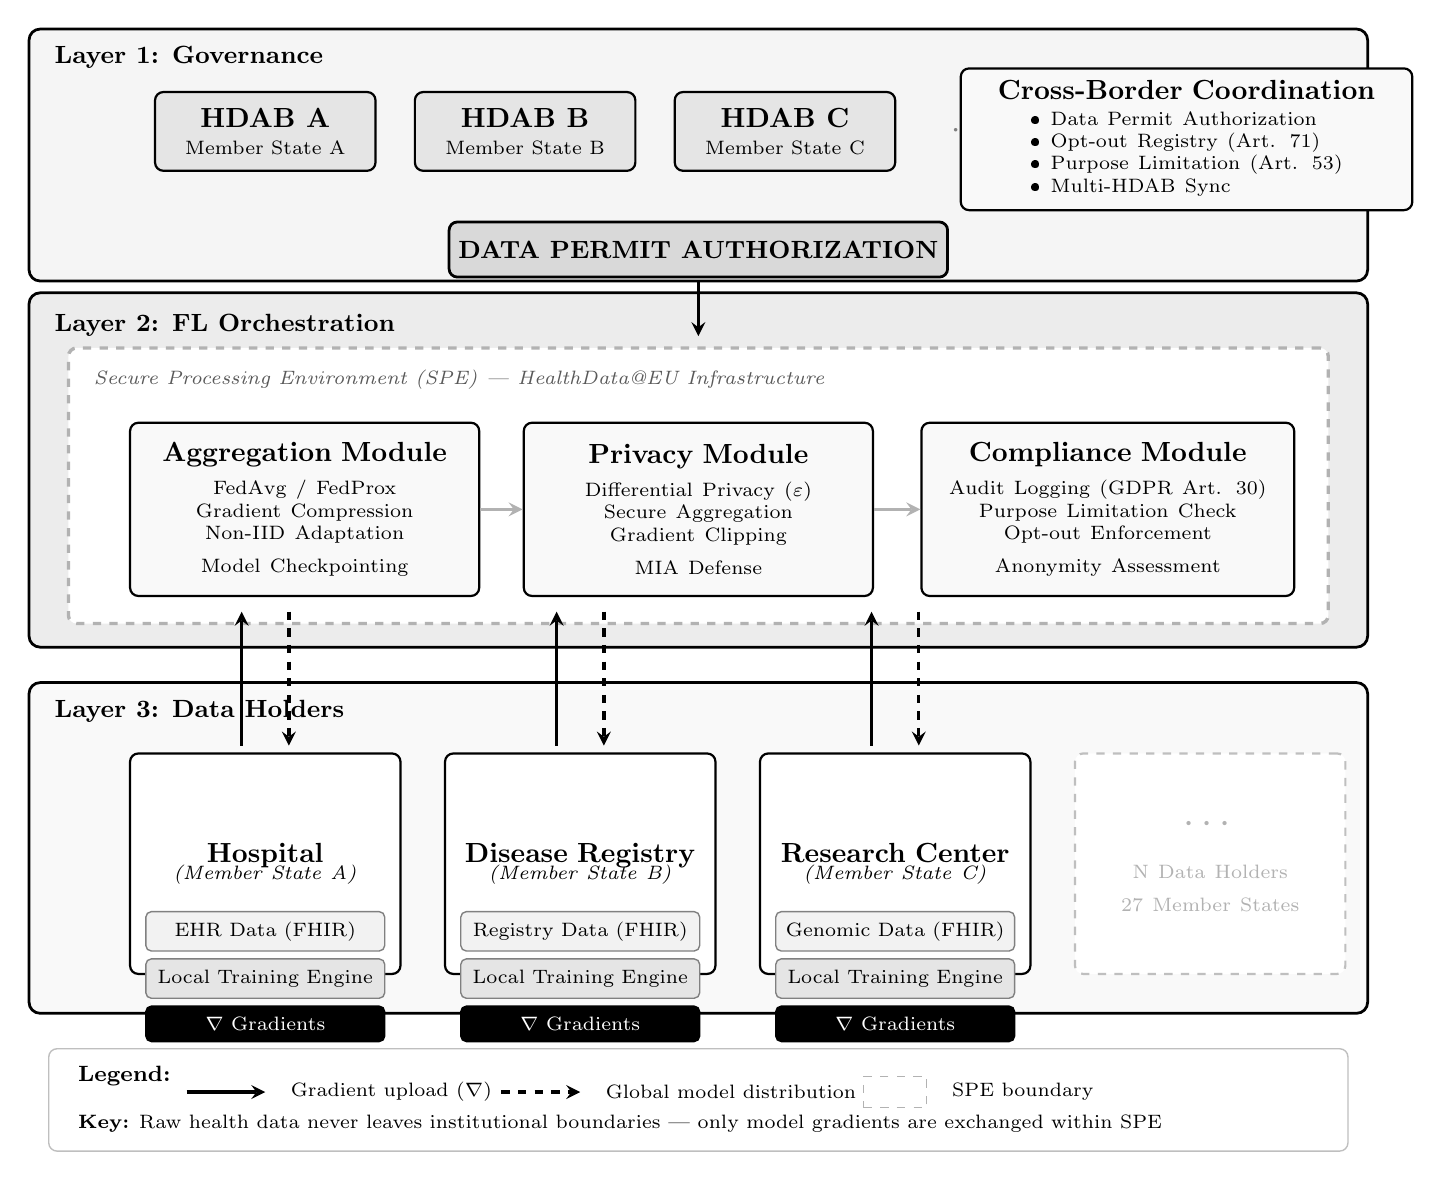
\begin{tikzpicture}[
    % Styles
    layer/.style={rectangle, rounded corners=4pt, minimum width=17cm, draw=black, line width=1pt},
    module/.style={rectangle, rounded corners=3pt, draw=black, line width=0.8pt, fill=white, minimum height=2.2cm, text width=4.2cm, align=center},
    hdab/.style={rectangle, rounded corners=3pt, draw=black, line width=0.8pt, fill=gray!20, minimum height=1cm, minimum width=2.8cm, align=center},
    dataholder/.style={rectangle, rounded corners=3pt, draw=black, line width=0.8pt, fill=white, minimum height=2.8cm, text width=3.2cm, align=center},
    databox/.style={rectangle, rounded corners=2pt, draw=gray, line width=0.5pt, fill=gray!10, minimum height=0.5cm, text width=2.8cm, align=center, font=\scriptsize},
    gradientbox/.style={rectangle, rounded corners=2pt, draw=black, line width=0.5pt, fill=black, minimum height=0.45cm, text width=2.8cm, align=center, font=\scriptsize\color{white}},
    arrow/.style={->, >=stealth, line width=1.2pt},
    dashedarrow/.style={->, >=stealth, line width=1.2pt, dashed},
    label/.style={font=\footnotesize},
    title/.style={font=\small\bfseries},
    subtitle/.style={font=\scriptsize\itshape, text=gray!70!black},
]

% ===== LAYER 1: GOVERNANCE =====
\node[layer, fill=gray!8, minimum height=3.2cm] (layer1) at (0, 8) {};
\node[title, anchor=north west] at (-8.3, 9.5) {Layer 1: Governance};

% HDABs
\node[hdab] (hdabA) at (-5.5, 8.3) {\textbf{HDAB A}\\[-2pt]\scriptsize Member State A};
\node[hdab] (hdabB) at (-2.2, 8.3) {\textbf{HDAB B}\\[-2pt]\scriptsize Member State B};
\node[hdab] (hdabC) at (1.1, 8.3) {\textbf{HDAB C}\\[-2pt]\scriptsize Member State C};
\node[font=\large, text=gray] at (3.5, 8.3) {$\cdots$};

% Coordination box
\node[module, minimum height=1.8cm, text width=5.5cm, fill=gray!5] (coord) at (6.2, 8.2) {
    \textbf{Cross-Border Coordination}\\[3pt]
    \scriptsize
    \begin{tabular}{@{}l@{}}
    • Data Permit Authorization\\
    • Opt-out Registry (Art. 71)\\
    • Purpose Limitation (Art. 53)\\
    • Multi-HDAB Sync
    \end{tabular}
};

% Data Permit box
\node[rectangle, rounded corners=3pt, draw=black, line width=1pt, fill=gray!30, minimum height=0.7cm, minimum width=5cm] (permit) at (0, 6.8) {\small\textbf{DATA PERMIT AUTHORIZATION}};

% ===== LAYER 2: FL ORCHESTRATION =====
\node[layer, fill=gray!15, minimum height=4.5cm] (layer2) at (0, 4) {};
\node[title, anchor=north west] at (-8.3, 6.1) {Layer 2: FL Orchestration};

% SPE boundary
\node[rectangle, rounded corners=3pt, draw=gray!60, line width=1.2pt, dashed, minimum width=16cm, minimum height=3.5cm, fill=white] (spe) at (0, 3.8) {};
\node[subtitle, anchor=north west] at (-7.8, 5.4) {Secure Processing Environment (SPE) — HealthData@EU Infrastructure};

% Modules
\node[module, fill=gray!5] (agg) at (-5, 3.5) {
    \textbf{Aggregation Module}\\[4pt]
    \scriptsize
    FedAvg / FedProx\\
    Gradient Compression\\
    Non-IID Adaptation\\
    Model Checkpointing
};

\node[module, fill=gray!5] (priv) at (0, 3.5) {
    \textbf{Privacy Module}\\[4pt]
    \scriptsize
    Differential Privacy ($\varepsilon$)\\
    Secure Aggregation\\
    Gradient Clipping\\
    MIA Defense
};

\node[module, fill=gray!5, text width=4.5cm] (comp) at (5.2, 3.5) {
    \textbf{Compliance Module}\\[4pt]
    \scriptsize
    Audit Logging (GDPR Art. 30)\\
    Purpose Limitation Check\\
    Opt-out Enforcement\\
    Anonymity Assessment
};

% Arrows between modules
\draw[arrow, gray!60] (agg.east) -- (priv.west);
\draw[arrow, gray!60] (priv.east) -- (comp.west);

% ===== LAYER 3: DATA HOLDERS =====
\node[layer, fill=gray!5, minimum height=4.2cm] (layer3) at (0, -0.8) {};
\node[title, anchor=north west] at (-8.3, 1.2) {Layer 3: Data Holders};

% Data holders
\node[dataholder] (hosp) at (-5.5, -1) {
    \textbf{Hospital}\\[-2pt]
    \scriptsize\textit{(Member State A)}\\[6pt]
};
\node[databox, anchor=north] at (-5.5, -1.6) {EHR Data (FHIR)};
\node[databox, anchor=north, fill=gray!20] at (-5.5, -2.2) {Local Training Engine};
\node[gradientbox, anchor=north] at (-5.5, -2.8) {$\nabla$ Gradients};

\node[dataholder] (reg) at (-1.5, -1) {
    \textbf{Disease Registry}\\[-2pt]
    \scriptsize\textit{(Member State B)}\\[6pt]
};
\node[databox, anchor=north] at (-1.5, -1.6) {Registry Data (FHIR)};
\node[databox, anchor=north, fill=gray!20] at (-1.5, -2.2) {Local Training Engine};
\node[gradientbox, anchor=north] at (-1.5, -2.8) {$\nabla$ Gradients};

\node[dataholder] (res) at (2.5, -1) {
    \textbf{Research Center}\\[-2pt]
    \scriptsize\textit{(Member State C)}\\[6pt]
};
\node[databox, anchor=north] at (2.5, -1.6) {Genomic Data (FHIR)};
\node[databox, anchor=north, fill=gray!20] at (2.5, -2.2) {Local Training Engine};
\node[gradientbox, anchor=north] at (2.5, -2.8) {$\nabla$ Gradients};

% More nodes indicator
\node[dataholder, draw=gray!50, dashed, text=gray!60] (more) at (6.5, -1) {
    \Large$\cdots$\\[8pt]
    \scriptsize N Data Holders\\
    27 Member States
};

% ===== DATA FLOW ARROWS =====
% Gradients up (solid)
\draw[arrow] (-5.8, 0.5) -- (-5.8, 2.2) node[midway, left, font=\tiny] {};
\draw[arrow] (-1.8, 0.5) -- (-1.8, 2.2);
\draw[arrow] (2.2, 0.5) -- (2.2, 2.2);

% Model down (dashed)
\draw[dashedarrow] (-5.2, 2.2) -- (-5.2, 0.5);
\draw[dashedarrow] (-1.2, 2.2) -- (-1.2, 0.5);
\draw[dashedarrow] (2.8, 2.2) -- (2.8, 0.5);

% Layer 1 to Layer 2
\draw[arrow] (0, 6.4) -- (0, 5.7);

% ===== LEGEND =====
\node[rectangle, rounded corners=3pt, draw=gray!50, line width=0.5pt, fill=white, minimum width=16.5cm, minimum height=1.3cm] at (0, -4) {};
\node[font=\footnotesize\bfseries, anchor=west] at (-8, -3.7) {Legend:};

% Gradient arrow
\draw[arrow] (-6.5, -3.9) -- (-5.5, -3.9);
\node[font=\scriptsize, anchor=west] at (-5.3, -3.9) {Gradient upload ($\nabla$)};

% Model arrow  
\draw[dashedarrow] (-2.5, -3.9) -- (-1.5, -3.9);
\node[font=\scriptsize, anchor=west] at (-1.3, -3.9) {Global model distribution};

% SPE
\node[rectangle, draw=gray!60, dashed, minimum width=0.8cm, minimum height=0.4cm] at (2.5, -3.9) {};
\node[font=\scriptsize, anchor=west] at (3.1, -3.9) {SPE boundary};

% Key principle
\node[font=\scriptsize, anchor=west] at (-8, -4.3) {\textbf{Key:} Raw health data never leaves institutional boundaries — only model gradients are exchanged within SPE};

\end{tikzpicture}
\caption{FL-EHDS three-layer compliance framework architecture. Layer~1 (Governance) integrates Health Data Access Bodies for cross-border data permit authorization and opt-out registry consultation per Article~71. Layer~2 (FL Orchestration) operates within a Secure Processing Environment, implementing gradient aggregation with FedAvg/FedProx, privacy protection via differential privacy and secure aggregation, and GDPR-compliant audit logging. Layer~3 (Data Holders) maintains raw data within institutional boundaries across 27 Member States; only gradients ($\nabla$) are transmitted upward while global model parameters flow downward.}
\label{fig:architecture}
\end{figure*}


\begin{figure*}[htbp]
\centering
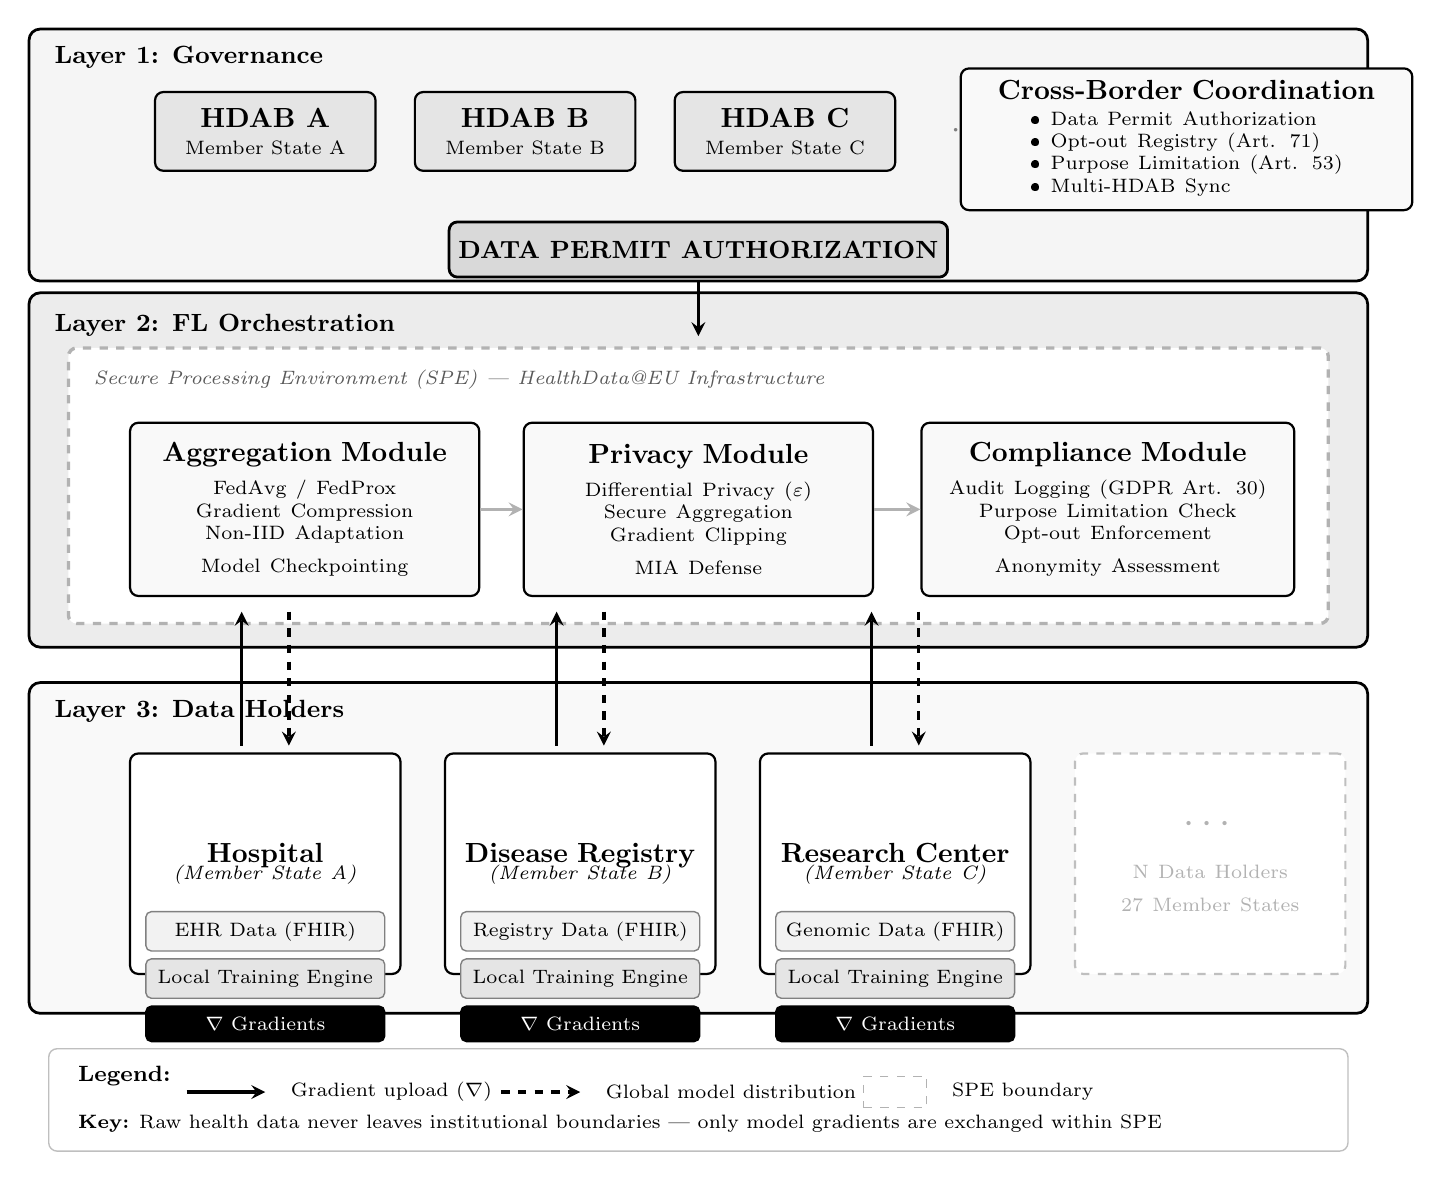
\begin{tikzpicture}[
    % Styles
    layer/.style={rectangle, rounded corners=4pt, minimum width=17cm, draw=black, line width=1pt},
    module/.style={rectangle, rounded corners=3pt, draw=black, line width=0.8pt, fill=white, minimum height=2.2cm, text width=4.2cm, align=center},
    hdab/.style={rectangle, rounded corners=3pt, draw=black, line width=0.8pt, fill=gray!20, minimum height=1cm, minimum width=2.8cm, align=center},
    dataholder/.style={rectangle, rounded corners=3pt, draw=black, line width=0.8pt, fill=white, minimum height=2.8cm, text width=3.2cm, align=center},
    databox/.style={rectangle, rounded corners=2pt, draw=gray, line width=0.5pt, fill=gray!10, minimum height=0.5cm, text width=2.8cm, align=center, font=\scriptsize},
    gradientbox/.style={rectangle, rounded corners=2pt, draw=black, line width=0.5pt, fill=black, minimum height=0.45cm, text width=2.8cm, align=center, font=\scriptsize\color{white}},
    arrow/.style={->, >=stealth, line width=1.2pt},
    dashedarrow/.style={->, >=stealth, line width=1.2pt, dashed},
    label/.style={font=\footnotesize},
    title/.style={font=\small\bfseries},
    subtitle/.style={font=\scriptsize\itshape, text=gray!70!black},
]

% ===== LAYER 1: GOVERNANCE =====
\node[layer, fill=gray!8, minimum height=3.2cm] (layer1) at (0, 8) {};
\node[title, anchor=north west] at (-8.3, 9.5) {Layer 1: Governance};

% HDABs
\node[hdab] (hdabA) at (-5.5, 8.3) {\textbf{HDAB A}\\[-2pt]\scriptsize Member State A};
\node[hdab] (hdabB) at (-2.2, 8.3) {\textbf{HDAB B}\\[-2pt]\scriptsize Member State B};
\node[hdab] (hdabC) at (1.1, 8.3) {\textbf{HDAB C}\\[-2pt]\scriptsize Member State C};
\node[font=\large, text=gray] at (3.5, 8.3) {$\cdots$};

% Coordination box
\node[module, minimum height=1.8cm, text width=5.5cm, fill=gray!5] (coord) at (6.2, 8.2) {
    \textbf{Cross-Border Coordination}\\[3pt]
    \scriptsize
    \begin{tabular}{@{}l@{}}
    • Data Permit Authorization\\
    • Opt-out Registry (Art. 71)\\
    • Purpose Limitation (Art. 53)\\
    • Multi-HDAB Sync
    \end{tabular}
};

% Data Permit box
\node[rectangle, rounded corners=3pt, draw=black, line width=1pt, fill=gray!30, minimum height=0.7cm, minimum width=5cm] (permit) at (0, 6.8) {\small\textbf{DATA PERMIT AUTHORIZATION}};

% ===== LAYER 2: FL ORCHESTRATION =====
\node[layer, fill=gray!15, minimum height=4.5cm] (layer2) at (0, 4) {};
\node[title, anchor=north west] at (-8.3, 6.1) {Layer 2: FL Orchestration};

% SPE boundary
\node[rectangle, rounded corners=3pt, draw=gray!60, line width=1.2pt, dashed, minimum width=16cm, minimum height=3.5cm, fill=white] (spe) at (0, 3.8) {};
\node[subtitle, anchor=north west] at (-7.8, 5.4) {Secure Processing Environment (SPE) — HealthData@EU Infrastructure};

% Modules
\node[module, fill=gray!5] (agg) at (-5, 3.5) {
    \textbf{Aggregation Module}\\[4pt]
    \scriptsize
    FedAvg / FedProx\\
    Gradient Compression\\
    Non-IID Adaptation\\
    Model Checkpointing
};

\node[module, fill=gray!5] (priv) at (0, 3.5) {
    \textbf{Privacy Module}\\[4pt]
    \scriptsize
    Differential Privacy ($\varepsilon$)\\
    Secure Aggregation\\
    Gradient Clipping\\
    MIA Defense
};

\node[module, fill=gray!5, text width=4.5cm] (comp) at (5.2, 3.5) {
    \textbf{Compliance Module}\\[4pt]
    \scriptsize
    Audit Logging (GDPR Art. 30)\\
    Purpose Limitation Check\\
    Opt-out Enforcement\\
    Anonymity Assessment
};

% Arrows between modules
\draw[arrow, gray!60] (agg.east) -- (priv.west);
\draw[arrow, gray!60] (priv.east) -- (comp.west);

% ===== LAYER 3: DATA HOLDERS =====
\node[layer, fill=gray!5, minimum height=4.2cm] (layer3) at (0, -0.8) {};
\node[title, anchor=north west] at (-8.3, 1.2) {Layer 3: Data Holders};

% Data holders
\node[dataholder] (hosp) at (-5.5, -1) {
    \textbf{Hospital}\\[-2pt]
    \scriptsize\textit{(Member State A)}\\[6pt]
};
\node[databox, anchor=north] at (-5.5, -1.6) {EHR Data (FHIR)};
\node[databox, anchor=north, fill=gray!20] at (-5.5, -2.2) {Local Training Engine};
\node[gradientbox, anchor=north] at (-5.5, -2.8) {$\nabla$ Gradients};

\node[dataholder] (reg) at (-1.5, -1) {
    \textbf{Disease Registry}\\[-2pt]
    \scriptsize\textit{(Member State B)}\\[6pt]
};
\node[databox, anchor=north] at (-1.5, -1.6) {Registry Data (FHIR)};
\node[databox, anchor=north, fill=gray!20] at (-1.5, -2.2) {Local Training Engine};
\node[gradientbox, anchor=north] at (-1.5, -2.8) {$\nabla$ Gradients};

\node[dataholder] (res) at (2.5, -1) {
    \textbf{Research Center}\\[-2pt]
    \scriptsize\textit{(Member State C)}\\[6pt]
};
\node[databox, anchor=north] at (2.5, -1.6) {Genomic Data (FHIR)};
\node[databox, anchor=north, fill=gray!20] at (2.5, -2.2) {Local Training Engine};
\node[gradientbox, anchor=north] at (2.5, -2.8) {$\nabla$ Gradients};

% More nodes indicator
\node[dataholder, draw=gray!50, dashed, text=gray!60] (more) at (6.5, -1) {
    \Large$\cdots$\\[8pt]
    \scriptsize N Data Holders\\
    27 Member States
};

% ===== DATA FLOW ARROWS =====
% Gradients up (solid)
\draw[arrow] (-5.8, 0.5) -- (-5.8, 2.2) node[midway, left, font=\tiny] {};
\draw[arrow] (-1.8, 0.5) -- (-1.8, 2.2);
\draw[arrow] (2.2, 0.5) -- (2.2, 2.2);

% Model down (dashed)
\draw[dashedarrow] (-5.2, 2.2) -- (-5.2, 0.5);
\draw[dashedarrow] (-1.2, 2.2) -- (-1.2, 0.5);
\draw[dashedarrow] (2.8, 2.2) -- (2.8, 0.5);

% Layer 1 to Layer 2
\draw[arrow] (0, 6.4) -- (0, 5.7);

% ===== LEGEND =====
\node[rectangle, rounded corners=3pt, draw=gray!50, line width=0.5pt, fill=white, minimum width=16.5cm, minimum height=1.3cm] at (0, -4) {};
\node[font=\footnotesize\bfseries, anchor=west] at (-8, -3.7) {Legend:};

% Gradient arrow
\draw[arrow] (-6.5, -3.9) -- (-5.5, -3.9);
\node[font=\scriptsize, anchor=west] at (-5.3, -3.9) {Gradient upload ($\nabla$)};

% Model arrow  
\draw[dashedarrow] (-2.5, -3.9) -- (-1.5, -3.9);
\node[font=\scriptsize, anchor=west] at (-1.3, -3.9) {Global model distribution};

% SPE
\node[rectangle, draw=gray!60, dashed, minimum width=0.8cm, minimum height=0.4cm] at (2.5, -3.9) {};
\node[font=\scriptsize, anchor=west] at (3.1, -3.9) {SPE boundary};

% Key principle
\node[font=\scriptsize, anchor=west] at (-8, -4.3) {\textbf{Key:} Raw health data never leaves institutional boundaries — only model gradients are exchanged within SPE};

\end{tikzpicture}
\caption{FL-EHDS three-layer compliance framework architecture. Layer~1 (Governance) integrates Health Data Access Bodies for cross-border data permit authorization and opt-out registry consultation per Article~71. Layer~2 (FL Orchestration) operates within a Secure Processing Environment, implementing gradient aggregation with FedAvg/FedProx, privacy protection via differential privacy and secure aggregation, and GDPR-compliant audit logging. Layer~3 (Data Holders) maintains raw data within institutional boundaries across 27 Member States; only gradients ($\nabla$) are transmitted upward while global model parameters flow downward.}
\label{fig:architecture}
\end{figure*}


\begin{figure*}[htbp]
\centering
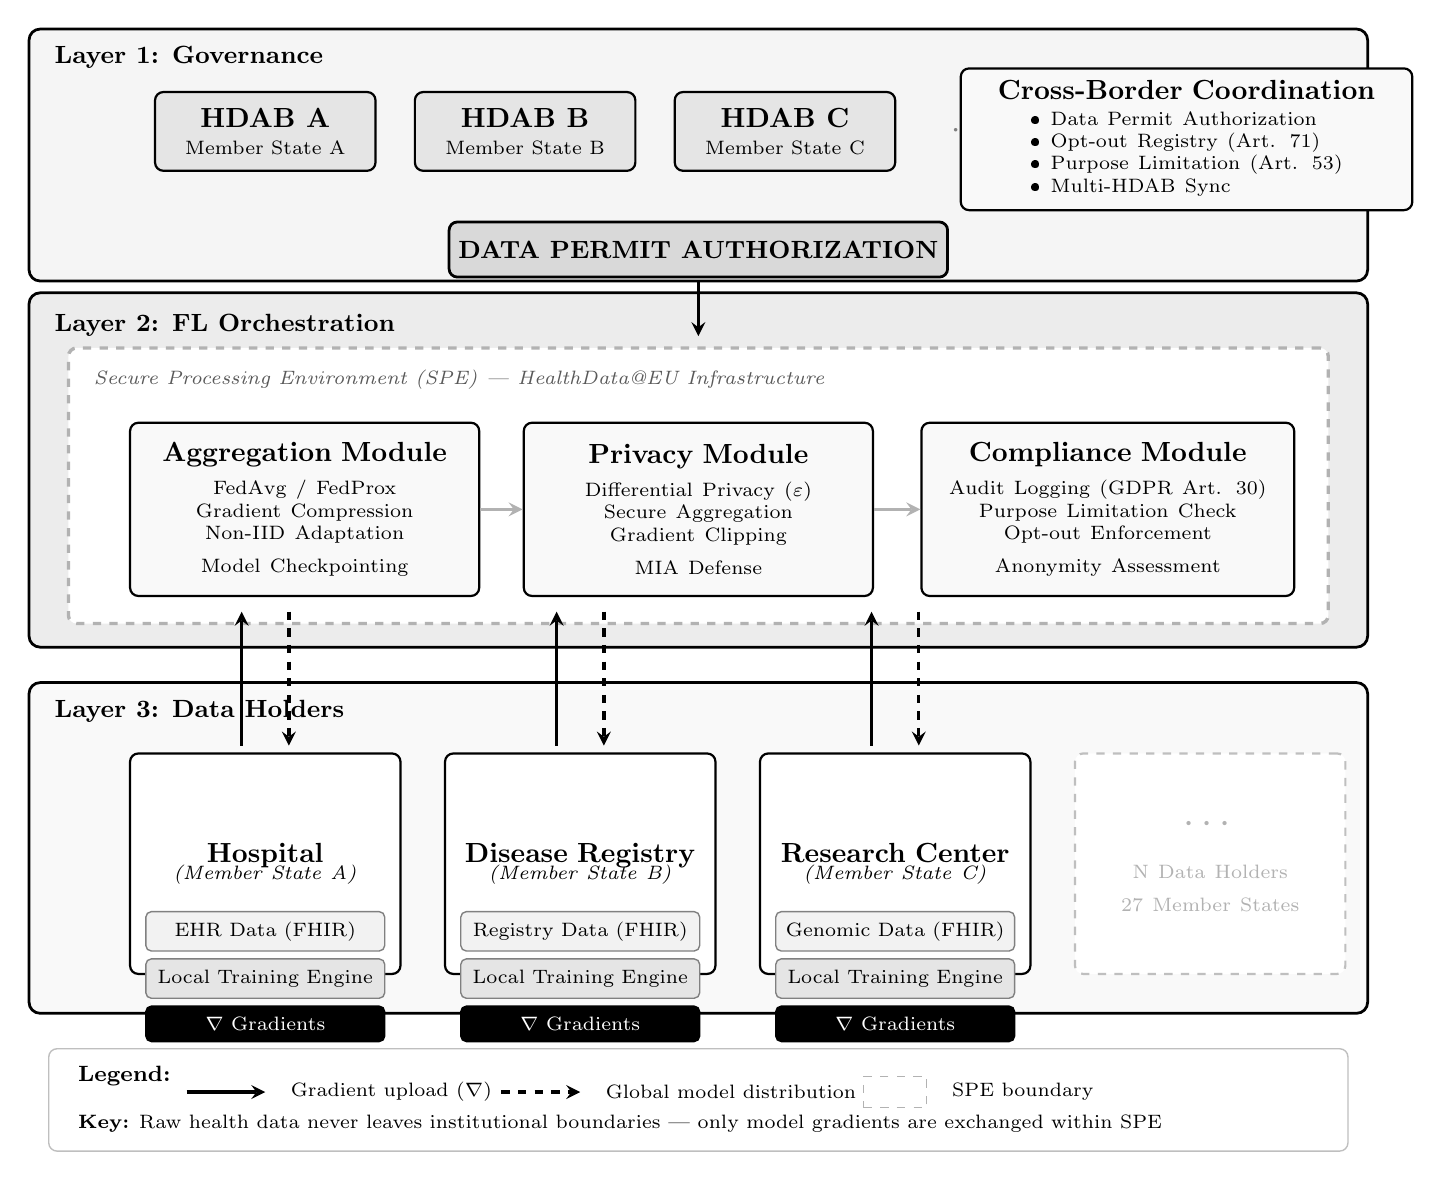
\begin{tikzpicture}[
    % Styles
    layer/.style={rectangle, rounded corners=4pt, minimum width=17cm, draw=black, line width=1pt},
    module/.style={rectangle, rounded corners=3pt, draw=black, line width=0.8pt, fill=white, minimum height=2.2cm, text width=4.2cm, align=center},
    hdab/.style={rectangle, rounded corners=3pt, draw=black, line width=0.8pt, fill=gray!20, minimum height=1cm, minimum width=2.8cm, align=center},
    dataholder/.style={rectangle, rounded corners=3pt, draw=black, line width=0.8pt, fill=white, minimum height=2.8cm, text width=3.2cm, align=center},
    databox/.style={rectangle, rounded corners=2pt, draw=gray, line width=0.5pt, fill=gray!10, minimum height=0.5cm, text width=2.8cm, align=center, font=\scriptsize},
    gradientbox/.style={rectangle, rounded corners=2pt, draw=black, line width=0.5pt, fill=black, minimum height=0.45cm, text width=2.8cm, align=center, font=\scriptsize\color{white}},
    arrow/.style={->, >=stealth, line width=1.2pt},
    dashedarrow/.style={->, >=stealth, line width=1.2pt, dashed},
    label/.style={font=\footnotesize},
    title/.style={font=\small\bfseries},
    subtitle/.style={font=\scriptsize\itshape, text=gray!70!black},
]

% ===== LAYER 1: GOVERNANCE =====
\node[layer, fill=gray!8, minimum height=3.2cm] (layer1) at (0, 8) {};
\node[title, anchor=north west] at (-8.3, 9.5) {Layer 1: Governance};

% HDABs
\node[hdab] (hdabA) at (-5.5, 8.3) {\textbf{HDAB A}\\[-2pt]\scriptsize Member State A};
\node[hdab] (hdabB) at (-2.2, 8.3) {\textbf{HDAB B}\\[-2pt]\scriptsize Member State B};
\node[hdab] (hdabC) at (1.1, 8.3) {\textbf{HDAB C}\\[-2pt]\scriptsize Member State C};
\node[font=\large, text=gray] at (3.5, 8.3) {$\cdots$};

% Coordination box
\node[module, minimum height=1.8cm, text width=5.5cm, fill=gray!5] (coord) at (6.2, 8.2) {
    \textbf{Cross-Border Coordination}\\[3pt]
    \scriptsize
    \begin{tabular}{@{}l@{}}
    • Data Permit Authorization\\
    • Opt-out Registry (Art. 71)\\
    • Purpose Limitation (Art. 53)\\
    • Multi-HDAB Sync
    \end{tabular}
};

% Data Permit box
\node[rectangle, rounded corners=3pt, draw=black, line width=1pt, fill=gray!30, minimum height=0.7cm, minimum width=5cm] (permit) at (0, 6.8) {\small\textbf{DATA PERMIT AUTHORIZATION}};

% ===== LAYER 2: FL ORCHESTRATION =====
\node[layer, fill=gray!15, minimum height=4.5cm] (layer2) at (0, 4) {};
\node[title, anchor=north west] at (-8.3, 6.1) {Layer 2: FL Orchestration};

% SPE boundary
\node[rectangle, rounded corners=3pt, draw=gray!60, line width=1.2pt, dashed, minimum width=16cm, minimum height=3.5cm, fill=white] (spe) at (0, 3.8) {};
\node[subtitle, anchor=north west] at (-7.8, 5.4) {Secure Processing Environment (SPE) — HealthData@EU Infrastructure};

% Modules
\node[module, fill=gray!5] (agg) at (-5, 3.5) {
    \textbf{Aggregation Module}\\[4pt]
    \scriptsize
    FedAvg / FedProx\\
    Gradient Compression\\
    Non-IID Adaptation\\
    Model Checkpointing
};

\node[module, fill=gray!5] (priv) at (0, 3.5) {
    \textbf{Privacy Module}\\[4pt]
    \scriptsize
    Differential Privacy ($\varepsilon$)\\
    Secure Aggregation\\
    Gradient Clipping\\
    MIA Defense
};

\node[module, fill=gray!5, text width=4.5cm] (comp) at (5.2, 3.5) {
    \textbf{Compliance Module}\\[4pt]
    \scriptsize
    Audit Logging (GDPR Art. 30)\\
    Purpose Limitation Check\\
    Opt-out Enforcement\\
    Anonymity Assessment
};

% Arrows between modules
\draw[arrow, gray!60] (agg.east) -- (priv.west);
\draw[arrow, gray!60] (priv.east) -- (comp.west);

% ===== LAYER 3: DATA HOLDERS =====
\node[layer, fill=gray!5, minimum height=4.2cm] (layer3) at (0, -0.8) {};
\node[title, anchor=north west] at (-8.3, 1.2) {Layer 3: Data Holders};

% Data holders
\node[dataholder] (hosp) at (-5.5, -1) {
    \textbf{Hospital}\\[-2pt]
    \scriptsize\textit{(Member State A)}\\[6pt]
};
\node[databox, anchor=north] at (-5.5, -1.6) {EHR Data (FHIR)};
\node[databox, anchor=north, fill=gray!20] at (-5.5, -2.2) {Local Training Engine};
\node[gradientbox, anchor=north] at (-5.5, -2.8) {$\nabla$ Gradients};

\node[dataholder] (reg) at (-1.5, -1) {
    \textbf{Disease Registry}\\[-2pt]
    \scriptsize\textit{(Member State B)}\\[6pt]
};
\node[databox, anchor=north] at (-1.5, -1.6) {Registry Data (FHIR)};
\node[databox, anchor=north, fill=gray!20] at (-1.5, -2.2) {Local Training Engine};
\node[gradientbox, anchor=north] at (-1.5, -2.8) {$\nabla$ Gradients};

\node[dataholder] (res) at (2.5, -1) {
    \textbf{Research Center}\\[-2pt]
    \scriptsize\textit{(Member State C)}\\[6pt]
};
\node[databox, anchor=north] at (2.5, -1.6) {Genomic Data (FHIR)};
\node[databox, anchor=north, fill=gray!20] at (2.5, -2.2) {Local Training Engine};
\node[gradientbox, anchor=north] at (2.5, -2.8) {$\nabla$ Gradients};

% More nodes indicator
\node[dataholder, draw=gray!50, dashed, text=gray!60] (more) at (6.5, -1) {
    \Large$\cdots$\\[8pt]
    \scriptsize N Data Holders\\
    27 Member States
};

% ===== DATA FLOW ARROWS =====
% Gradients up (solid)
\draw[arrow] (-5.8, 0.5) -- (-5.8, 2.2) node[midway, left, font=\tiny] {};
\draw[arrow] (-1.8, 0.5) -- (-1.8, 2.2);
\draw[arrow] (2.2, 0.5) -- (2.2, 2.2);

% Model down (dashed)
\draw[dashedarrow] (-5.2, 2.2) -- (-5.2, 0.5);
\draw[dashedarrow] (-1.2, 2.2) -- (-1.2, 0.5);
\draw[dashedarrow] (2.8, 2.2) -- (2.8, 0.5);

% Layer 1 to Layer 2
\draw[arrow] (0, 6.4) -- (0, 5.7);

% ===== LEGEND =====
\node[rectangle, rounded corners=3pt, draw=gray!50, line width=0.5pt, fill=white, minimum width=16.5cm, minimum height=1.3cm] at (0, -4) {};
\node[font=\footnotesize\bfseries, anchor=west] at (-8, -3.7) {Legend:};

% Gradient arrow
\draw[arrow] (-6.5, -3.9) -- (-5.5, -3.9);
\node[font=\scriptsize, anchor=west] at (-5.3, -3.9) {Gradient upload ($\nabla$)};

% Model arrow  
\draw[dashedarrow] (-2.5, -3.9) -- (-1.5, -3.9);
\node[font=\scriptsize, anchor=west] at (-1.3, -3.9) {Global model distribution};

% SPE
\node[rectangle, draw=gray!60, dashed, minimum width=0.8cm, minimum height=0.4cm] at (2.5, -3.9) {};
\node[font=\scriptsize, anchor=west] at (3.1, -3.9) {SPE boundary};

% Key principle
\node[font=\scriptsize, anchor=west] at (-8, -4.3) {\textbf{Key:} Raw health data never leaves institutional boundaries — only model gradients are exchanged within SPE};

\end{tikzpicture}
\caption{FL-EHDS three-layer compliance framework architecture. Layer~1 (Governance) integrates Health Data Access Bodies for cross-border data permit authorization and opt-out registry consultation per Article~71. Layer~2 (FL Orchestration) operates within a Secure Processing Environment, implementing gradient aggregation with FedAvg/FedProx, privacy protection via differential privacy and secure aggregation, and GDPR-compliant audit logging. Layer~3 (Data Holders) maintains raw data within institutional boundaries across 27 Member States; only gradients ($\nabla$) are transmitted upward while global model parameters flow downward.}
\label{fig:architecture}
\end{figure*}


\subsection{Layer 1: Governance}

Standardized APIs enable automated data permit verification before FL training initiation. Multi-HDAB synchronization protocols coordinate cross-border studies involving multiple Member States, addressing the coordination complexity identified by Christiansen et al.~\cite{christiansen2025pilot}. National opt-out registries are consulted before each training round, ensuring Article~71 compliance at record-level granularity. Comprehensive audit trails satisfy GDPR Article~30 requirements, documenting data access, processing purposes, and model outputs for regulatory inspection.

Algorithm~1 presents the core FL-EHDS training procedure, highlighting governance checkpoints integrated into each round.

\begin{figure}[htbp]
\centering
\fbox{\parbox{0.92\columnwidth}{
\small
\textbf{Algorithm 1: FL-EHDS FedAvg Training}\\[2pt]
\textbf{Input:} Hospitals $\mathcal{H} = \{h_1, \ldots, h_K\}$, permit $P$, rounds $T$\\
\textbf{Output:} Global model $\theta^{(T)}$\\[3pt]
\textbf{Server executes:}\\
\hspace*{4mm}Initialize $\theta^{(0)}$\\
\hspace*{4mm}\textbf{for} round $t = 1$ to $T$ \textbf{do}\\
\hspace*{8mm}\textit{// Governance check (Layer 1)}\\
\hspace*{8mm}\textbf{if} not ValidatePermit($P$, $t$) \textbf{then abort}\\
\hspace*{8mm}$\mathcal{H}_t \leftarrow$ SelectParticipants($\mathcal{H}$)\\
\hspace*{8mm}\textbf{for each} $h \in \mathcal{H}_t$ \textbf{in parallel do}\\
\hspace*{12mm}$\Delta_h^{(t)}, n_h \leftarrow$ LocalTrain($h$, $\theta^{(t-1)}$)\\
\hspace*{8mm}\textit{// Aggregation with privacy (Layer 2)}\\
\hspace*{8mm}$\theta^{(t)} \leftarrow \theta^{(t-1)} + \frac{1}{\sum n_h} \sum_{h} n_h \cdot \Delta_h^{(t)}$\\
\hspace*{8mm}LogCompliance($t$, $\mathcal{H}_t$)\\[3pt]
\textbf{LocalTrain}($h$, $\theta$):\\
\hspace*{4mm}$\mathcal{D}_h \leftarrow$ FilterOptedOut($\mathcal{D}_h$, Registry) \textit{// Art.~71}\\
\hspace*{4mm}$\theta_h \leftarrow \theta$; train $E$ epochs on $\mathcal{D}_h$\\
\hspace*{4mm}$\Delta_h \leftarrow$ ClipGradient($\theta_h - \theta$, $C$) \textit{// DP bound}\\
\hspace*{4mm}\textbf{return} $\Delta_h$, $|\mathcal{D}_h|$
}}
\end{figure}

\subsection{Layer 2: FL Orchestration}

The framework implements \textbf{17 aggregation algorithms} spanning six categories---from foundational methods (FedAvg~\cite{mcmahan2017communication}, FedProx~\cite{li2020federated}) through non-IID robustness (SCAFFOLD~\cite{karimireddy2020scaffold}, FedNova~\cite{wang2020tackling}, FedDyn~\cite{acar2021feddyn}), adaptive optimization~\cite{reddi2021adaptive}, and personalization (Ditto~\cite{li2021ditto}, Per-FedAvg~\cite{fallah2020personalized}) to the latest advances: FedLESAM~\cite{qu2024fedlesam} (ICML 2024 Spotlight) and HPFL~\cite{chen2025hpfl} (ICLR 2025). Table~\ref{tab:algo_catalogue} provides the complete catalogue with venues and key properties.

Two recent algorithms merit particular attention for EHDS scenarios. FedLESAM~\cite{qu2024fedlesam} extends sharpness-aware minimization~\cite{qu2022fedsam} by replacing local gradient perturbation with a globally-estimated direction, achieving stronger generalization across heterogeneous distributions---directly relevant where cross-border patient populations differ substantially. HPFL~\cite{chen2025hpfl} decouples feature extraction from classification by aggregating only backbone parameters while keeping client-specific classifier heads local, enabling per-institution specialization without compromising collaborative learning. Algorithm selection is configurable; composable strategies (FedLC~\cite{zhang2022fedlc}, FedDecorr~\cite{shi2023feddecorr}) can augment any base aggregation.

\begin{table}[htbp]
\centering
\caption{FL-EHDS Algorithm Catalogue (17 Algorithms)}
\label{tab:algo_catalogue}
\small
\begin{tabular}{llll}
\toprule
\textbf{Algorithm} & \textbf{Venue} & \textbf{Category} & \textbf{Key Property} \\
\midrule
FedAvg & AISTATS'17 & Baseline & Weighted avg. \\
FedProx & MLSys'20 & Non-IID & Proximal reg. \\
SCAFFOLD & ICML'20 & Non-IID & Variance red. \\
FedNova & NeurIPS'20 & Non-IID & Normalized avg. \\
FedDyn & ICLR'21 & Non-IID & Dynamic reg. \\
FedAdam & ICLR'21 & Adaptive & Server momentum \\
FedYogi & ICLR'21 & Adaptive & Sparse stability \\
FedAdagrad & ICLR'21 & Adaptive & Grad.\ accum. \\
Ditto & ICML'21 & Personal. & Dual models \\
Per-FedAvg & NeurIPS'20 & Personal. & MAML-based \\
FedLC & ICML'22 & Label skew & Logit calibration \\
FedSAM & ICML'22 & Generalize & Flat minima \\
FedDecorr & ICLR'23 & Represent. & Decorrelation \\
FedSpeed & ICLR'23 & Efficiency & Fewer rounds \\
FedExP & ICLR'23 & Server-side & POCS step size \\
\textbf{FedLESAM} & \textbf{ICML'24} & \textbf{Generalize} & \textbf{Global SAM} \\
\textbf{HPFL} & \textbf{ICLR'25} & \textbf{Personal.} & \textbf{Local classif.} \\
\bottomrule
\end{tabular}

\vspace{1mm}
\footnotesize{\textbf{Bold}: newly added algorithms (2024--2025). All 17 implemented in the open-source reference implementation.}
\end{table}

\textbf{Privacy Protection}: Differential privacy~\cite{dwork2014dp} with configurable $\varepsilon$-budget uses DP-SGD~\cite{abadi2016deep} with R\'enyi DP (RDP)~\cite{mironov2017renyi} for tight composition accounting over multiple training rounds~\cite{wei2020federated}. For Gaussian mechanisms with noise scale $\sigma$, the RDP guarantee at order $\alpha$ is $\rho(\alpha) = \alpha/(2\sigma^2)$. For 100+ round training typical of EHDS cross-border studies, RDP provides 5--6$\times$ tighter privacy bounds than naive composition~\cite{mironov2017renyi, wei2020federated}, enabling longer training with equivalent privacy guarantees. Gradient clipping bounds individual contributions; secure aggregation (pairwise masking protocol with ECDH key exchange) mitigates gradient inversion attacks~\cite{zhu2019deep}. Six Byzantine resilience methods (Krum, Multi-Krum, Trimmed Mean, Median, Bulyan, FLTrust) defend against up to $f < n/3$ malicious clients.

\textbf{Purpose Limitation}: Technical enforcement of Article~53 permitted purposes through model output filtering and use-case validation, preventing scope creep beyond authorized analytics.

\subsection{Layer 3: Data Holders}

Resource-aware training engines address hardware heterogeneity (78\% barrier prevalence). The engine dynamically adjusts batch sizes, model complexity, and synchronization frequency based on local computational capabilities, enabling participation of institutions with diverse hardware profiles---from GPU-equipped university hospitals to CPU-only rural clinics.

\textbf{FHIR Preprocessing}: Data normalization pipelines ensure interoperability across heterogeneous EHR systems. Only 34\% of European healthcare providers achieve full FHIR compliance~\cite{hussein2025interop}; the preprocessing module bridges format gaps through automated transformation pipelines supporting FHIR R4 resources (Patient, Observation, Condition, MedicationRequest, DiagnosticReport) with standard coding systems (SNOMED-CT, LOINC, ICD-10).

\textbf{Secure Communication}: End-to-end encrypted gradient transmission with certificate-based authentication ensures no raw data leaves institutional boundaries. The communication layer supports gRPC for model updates and WebSocket for real-time monitoring events.

\subsection{Threat Model}

The framework assumes an honest-but-curious aggregation server. Byzantine tolerance is provided for up to $f < n/3$ malicious clients through robust aggregation (Krum, Trimmed Mean, Bulyan). Gradient inversion is mitigated by DP and secure aggregation.

\subsection{EHDS Compliance Mapping}

Table~\ref{tab:compliance} maps framework components to EHDS regulatory requirements.

\begin{table}[htbp]
\caption{EHDS Compliance Mapping}
\label{tab:compliance}
\centering
\small
\begin{tabular}{lp{2.3cm}p{2.8cm}}
\toprule
\textbf{Article} & \textbf{Requirement} & \textbf{FL-EHDS Component} \\
\midrule
Art. 33 & Secondary use auth. & HDAB API + Permit valid. \\
Art. 46 & Cross-border proc. & Multi-HDAB coordinator \\
Art. 50 & Secure Proc.\ Env. & Aggregation within SPE \\
Art. 53 & Permitted purposes & Purpose limitation module \\
Art. 71 & Opt-out mechanism & Registry filtering \\
\bottomrule
\end{tabular}
\end{table}

\subsection{Reference Implementation}

A modular Python implementation is available as open-source software, designed following FAIR principles~\cite{chaverodiez2026fair} (findable via GitHub with DOI, accessible under MIT license, interoperable via PyTorch and FHIR R4 interfaces, reusable with comprehensive documentation). The codebase ($\sim$40K lines, 159 modules) provides: (1) orchestration modules implementing all 17 algorithms with RDP accounting and secure aggregation; (2) six Byzantine resilience methods; (3) data holder utilities for adaptive training and FHIR R4 preprocessing; (4) a Streamlit-based dashboard for interactive FL training, EHDS governance workflow, and real-time monitoring; (5) a professional terminal UI with 11 specialized screens; (6) reproducible benchmark suite generating all experimental results.

\textbf{Note on governance}: HDAB integration includes a fully functional simulation backend demonstrating the complete permit lifecycle (OAuth2/mTLS authentication, permit CRUD, cross-border coordination) and Article~71 opt-out compliance (LRU-cached registry lookups, scope-granular filtering). Production deployment will require binding to actual HDAB services (expected 2027--2029).

% ============================================================================
% 4. EXPERIMENTAL EVALUATION
% ============================================================================
\section{Experimental Evaluation}
\label{sec:experiments}

We evaluate FL-EHDS on real clinical datasets simulating cross-border healthcare analytics. All results are fully reproducible via the benchmark suite in the repository.

\subsection{Setup}

\textbf{Datasets}: We evaluate on 8 datasets spanning tabular EHR and medical imaging (Table~\ref{tab:dataset_coverage}). Tabular datasets cover three scale regimes: \textit{small-data FL} (Heart Disease UCI, 920 patients from 4 international hospitals with natural non-IID partitioning; Breast Cancer Wisconsin, 569 FNA pathology samples), \textit{medium-scale} (PTB-XL ECG, 21,799 European-origin records from 52 German recording sites with natural hospital partitioning and 5-class SCP-ECG diagnosis), and \textit{large-scale} (Diabetes 130-US, 101,766 encounters; Cardiovascular Disease, 70,000 patients). Imaging datasets include Chest X-ray (5,856, binary), Brain Tumor MRI (3,064, 4-class), and Skin Cancer (3,297, binary). The full 19-dataset framework landscape is detailed in Supplementary Material, Table~S1. \textbf{Model}: HealthcareMLP (2-layer, 64/32 hidden, ReLU, dropout 0.3, $\sim$10K parameters) for tabular; ResNet-18 ($\sim$11.2M parameters) for imaging. \textbf{Configuration}: Per-dataset optimized hyperparameters (see Supplementary Material, Table~S9): PTB-XL (lr=0.005, bs=64, 30 rounds), Cardiovascular (lr=0.01, bs=64, 25 rounds), Breast Cancer (lr=0.001, bs=16, 40 rounds, 1 local epoch to prevent overfitting on 569 samples). All other datasets use 3 local epochs. Adam optimizer throughout; early stopping with patience=6. All results are mean $\pm$ std over 5 seeds.

\begin{table}[htbp]
\centering
\caption{Evaluated Dataset Coverage}
\label{tab:dataset_coverage}
\resizebox{\columnwidth}{!}{%
\begin{tabular}{lcccl}
\toprule
\textbf{Dataset} & \textbf{Samples} & \textbf{Feat.} & \textbf{Cls.} & \textbf{FL Partition} \\
\midrule
\multicolumn{5}{l}{\textit{Tabular Clinical (MLP, $\sim$10K params)}} \\
Heart Disease UCI & 920 & 13 & 2 & Natural (4 hosp.) \\
Breast Cancer Wisc. & 569 & 30 & 2 & Dirichlet \\
PTB-XL ECG$^\dagger$ & 21,799 & 9 & 5 & Natural (52 EU sites) \\
Diabetes 130-US & 101,766 & 22 & 2 & Dirichlet \\
Cardiovascular & 70,000 & 11 & 2 & Dirichlet \\
\midrule
\multicolumn{5}{l}{\textit{Medical Imaging (ResNet-18, $\sim$11.2M params)}} \\
Chest X-ray & 5,856 & --- & 2 & Dirichlet \\
Brain Tumor MRI & 3,064 & --- & 4 & Dirichlet \\
Skin Cancer & 3,297 & --- & 2 & Dirichlet \\
\bottomrule
\end{tabular}%
}

\vspace{1mm}
\footnotesize{$^\dagger$European-origin (PTB, Berlin), SCP-ECG standard (EN 1064), 5-class cardiac diagnosis. The 52 recording sites are grouped into $K$ geographic clusters for FL experiments (default $K{=}5$); client scaling evaluates $K \in \{3, 5, 10, 20\}$ in Supplementary Material.}
\end{table}

\subsection{Algorithm Comparison}

Table~\ref{tab:main_results} presents FL algorithm comparison on Heart Disease and Diabetes. Table~\ref{tab:tabular_main} extends evaluation to PTB-XL, Cardiovascular, and Breast Cancer with 7 algorithms including FedLESAM and HPFL---1,410 total experiments across heterogeneity sweeps, client scaling, learning rate sensitivity, and differential privacy ablation (see Supplementary Material, Section~S11).

\begin{table}[htbp]
\centering
\caption{FL Algorithm Comparison on Real Clinical Datasets}
\label{tab:main_results}
\resizebox{\columnwidth}{!}{%
\begin{tabular}{lcccccc}
\toprule
& \multicolumn{3}{c}{\textbf{Heart Disease (4 hosp.)}} & \multicolumn{3}{c}{\textbf{Diabetes (5 hosp.)}} \\
\cmidrule(lr){2-4} \cmidrule(lr){5-7}
\textbf{Algo.} & \textbf{Acc.} & \textbf{F1} & \textbf{AUC} & \textbf{Acc.} & \textbf{F1} & \textbf{AUC} \\
\midrule
FedAvg       & 62.5$\pm$8.0 & .736$\pm$.06 & .834$\pm$.03 & 68.1$\pm$4.2 & .259$\pm$.01 & .643$\pm$.00 \\
FedProx      & 61.7$\pm$8.0 & .732$\pm$.05 & .834$\pm$.03 & 71.0$\pm$6.3 & .254$\pm$.01 & .638$\pm$.00 \\
SCAFFOLD     & 66.3$\pm$5.1 & .667$\pm$.02 & .791$\pm$.05 & 11.2$\pm$0.0 & .201$\pm$.00 & .514$\pm$.00 \\
FedNova      & 56.4$\pm$5.4 & .711$\pm$.04 & .831$\pm$.03 & 13.0$\pm$0.9 & .203$\pm$.00 & .636$\pm$.00 \\
\textbf{Ditto} & \textbf{75.1$\pm$2.0} & \textbf{.761$\pm$.03} & .826$\pm$.01 & \textbf{71.7$\pm$0.2} & \textbf{.262$\pm$.00} & \textbf{.643$\pm$.00} \\
\bottomrule
\end{tabular}%
}

\vspace{1mm}
\footnotesize{20 rounds, 3 local epochs. Heart Disease: natural non-IID. Diabetes: Dirichlet $\alpha$=0.5. Mean $\pm$ std over 5 seeds.}
\end{table}

\begin{table*}[htbp]
\centering
\caption{Extended FL Algorithm Comparison on Tabular Healthcare Datasets (7 Algorithms $\times$ 3 Datasets). Best accuracy per dataset in \textbf{bold}. Mean $\pm$ std over 5 seeds. PX = PTB-XL ECG (5 clients, 5-class, site-based), CV = Cardiovascular (5 clients, binary, $\alpha$=0.5), BC = Breast Cancer (3 clients, binary, $\alpha$=0.5).}
\label{tab:tabular_main}
\resizebox{\textwidth}{!}{%
\begin{tabular}{lccccccccc}
\toprule
\textbf{Algorithm} & \multicolumn{3}{c}{\textbf{PTB-XL ECG (21,799 records, 52 EU sites)}} & \multicolumn{3}{c}{\textbf{Cardiovascular (70K patients)}} & \multicolumn{3}{c}{\textbf{Breast Cancer (569 samples)}} \\
\cmidrule(lr){2-4}\cmidrule(lr){5-7}\cmidrule(lr){8-10}
 & Acc (\%) & F1 (\%) & Jain & Acc (\%) & F1 (\%) & Jain & Acc (\%) & F1 (\%) & Jain \\
\midrule
FedAvg & 91.9$\pm$0.5 & 100.0 & 0.999 & 71.1$\pm$1.8 & 68.8 & 0.981 & 52.3$\pm$17.9 & 32.0 & 0.608 \\
FedProx & 91.6$\pm$0.7 & 100.0 & 0.999 & 71.5$\pm$1.2 & 69.6 & 0.986 & 52.3$\pm$17.9 & 32.0 & 0.608 \\
\textbf{Ditto} & 91.8$\pm$0.3 & 99.3 & 0.999 & \textbf{82.5$\pm$4.7} & 82.3 & 0.980 & \textbf{79.1$\pm$12.5} & 64.5 & 0.606 \\
FedLC & 91.9$\pm$0.5 & 100.0 & 0.999 & 71.1$\pm$1.6 & 68.8 & 0.982 & 52.1$\pm$18.1 & 32.6 & 0.606 \\
FedExP & 92.0$\pm$0.2 & 100.0 & 0.999 & 71.1$\pm$1.8 & 68.8 & 0.981 & 52.3$\pm$17.9 & 32.0 & 0.608 \\
FedLESAM & 91.9$\pm$0.5 & 100.0 & 0.999 & 71.1$\pm$1.8 & 68.8 & 0.981 & 52.3$\pm$17.9 & 32.0 & 0.608 \\
\textbf{HPFL} & \textbf{92.5$\pm$0.3} & 100.0 & 0.999 & 82.3$\pm$4.5 & 82.0 & 0.984 & 74.1$\pm$20.9 & 62.1 & 0.867 \\
\bottomrule
\end{tabular}%
}
\end{table*}

\subsection{Convergence and Baselines}

Figure~\ref{fig:convergence} shows training convergence on Heart Disease. Ditto converges faster and higher due to personalized local models.

\begin{figure}[htbp]
\centering
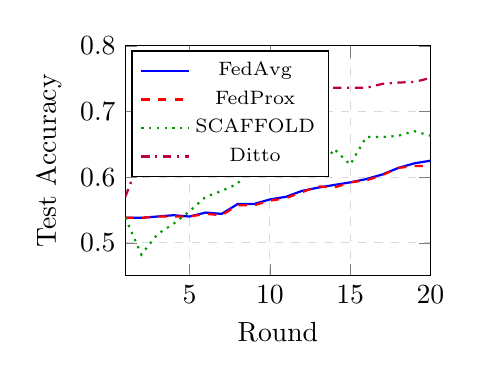
\begin{tikzpicture}
\begin{axis}[
    width=0.45\textwidth,
    height=4.5cm,
    xlabel={Round},
    ylabel={Test Accuracy},
    legend style={at={(0.02,0.98)}, anchor=north west, font=\scriptsize},
    grid=major,
    grid style={dashed, gray!30},
    xmin=1, xmax=20,
    ymin=0.45, ymax=0.80,
]
\addplot[blue, thick] coordinates {(1,0.538) (2,0.538) (3,0.540) (4,0.542) (5,0.540) (6,0.546) (7,0.544) (8,0.559) (9,0.559) (10,0.566) (11,0.570) (12,0.579) (13,0.584) (14,0.588) (15,0.592) (16,0.597) (17,0.604) (18,0.614) (19,0.621) (20,0.625)};
\addplot[red, thick, dashed] coordinates {(1,0.538) (2,0.538) (3,0.540) (4,0.540) (5,0.540) (6,0.544) (7,0.542) (8,0.557) (9,0.557) (10,0.564) (11,0.568) (12,0.577) (13,0.586) (14,0.584) (15,0.592) (16,0.595) (17,0.603) (18,0.614) (19,0.617) (20,0.617)};
\addplot[green!60!black, thick, dotted] coordinates {(1,0.538) (2,0.482) (3,0.513) (4,0.529) (5,0.548) (6,0.570) (7,0.579) (8,0.590) (9,0.625) (10,0.636) (11,0.628) (12,0.626) (13,0.604) (14,0.643) (15,0.619) (16,0.661) (17,0.661) (18,0.663) (19,0.670) (20,0.663)};
\addplot[purple, thick, dashdotted] coordinates {(1,0.570) (2,0.634) (3,0.667) (4,0.689) (5,0.696) (6,0.692) (7,0.705) (8,0.705) (9,0.712) (10,0.722) (11,0.727) (12,0.731) (13,0.736) (14,0.736) (15,0.736) (16,0.736) (17,0.742) (18,0.744) (19,0.745) (20,0.751)};
\legend{FedAvg, FedProx, SCAFFOLD, Ditto}
\end{axis}
\end{tikzpicture}
\caption{Training convergence on Heart Disease UCI (4 hospitals, natural non-IID). Ditto converges faster due to personalized local models.}
\label{fig:convergence}
\end{figure}

\textbf{Key findings}: Ditto converges to 75.1\% by round 20, compared to 62.5\% for FedAvg---a 12.6pp advantage. SCAFFOLD exhibits high variance (oscillating between 48\% and 66\%) due to control variate instability with only 4 heterogeneous clients. FedProx closely tracks FedAvg, suggesting that proximal regularization alone is insufficient for the degree of heterogeneity present.

Table~\ref{tab:fl_vs_central} compares three learning paradigms on Heart Disease, representing the EHDS deployment spectrum: centralized (upper bound, no privacy), federated (data stays local), and local-only (no collaboration).

\begin{table}[htbp]
\centering
\caption{Learning Paradigm Comparison (Heart Disease UCI)}
\label{tab:fl_vs_central}
\small
\begin{tabular}{lcccc}
\toprule
\textbf{Approach} & \textbf{Acc.} & \textbf{F1} & \textbf{AUC} & \textbf{Gap} \\
\midrule
Centralized & $81.7 \pm 2.9$\% & $.815$ & $.882$ & --- \\
FL-Ditto & $75.1 \pm 2.0$\% & $.761$ & $.826$ & 6.6pp \\
FL-FedAvg & $62.5 \pm 8.0$\% & $.736$ & $.834$ & 19.2pp \\
Local-Only$^*$ & $81.7 \pm 1.2$\% & $.797$ & --- & 0.0pp \\
\bottomrule
\end{tabular}

\vspace{1mm}
\footnotesize{4 hospitals, natural non-IID partitioning. Centralized/Local: 60 epochs, Adam (lr=0.01). FL: 20 rounds $\times$ 3 local epochs. Mean $\pm$ std over 5 seeds. $^*$Local-only evaluated on own test split (not cross-hospital).}
\end{table}

Centralized training achieves 81.7\% accuracy as expected. FL-Ditto narrows this gap to only \textbf{6.6pp} while preserving full data sovereignty---the strongest privacy-utility tradeoff among tested approaches. Baseline FedAvg suffers a 19.2pp gap, underscoring the importance of personalization-aware aggregation. Note that Local-Only accuracy (81.7\%) appears to match Centralized, but this comparison is misleading: Local-Only is evaluated only on each hospital's own test split (where it overfits to local distribution), whereas Centralized and FL approaches are evaluated on the pooled cross-hospital test set. Local-only models do not generalize: a model trained at the Swiss hospital performs poorly on Hungarian data. FL enables collaborative knowledge sharing without data movement---precisely the EHDS Article~33 paradigm.

\subsection{Non-IID Impact Analysis}

Figure~\ref{fig:noniid_impact} illustrates the impact of data heterogeneity on algorithm performance. As non-IID severity increases ($\alpha \to 0$), algorithm selection becomes increasingly critical---variance-reduction methods maintain stability while baseline FedAvg degrades significantly.

\begin{figure}[htbp]
\centering
\includegraphics[width=0.95\columnwidth]{figures/fig_accuracy_vs_noniid.pdf}
\caption{Final accuracy vs.\ data heterogeneity level (Dirichlet $\alpha$). Algorithm choice becomes critical as non-IID severity grows.}
\label{fig:noniid_impact}
\end{figure}

\subsection{Per-Hospital Heterogeneity}

Figure~\ref{fig:client_heterogeneity} shows per-hospital accuracy variation on Heart Disease, where the four hospitals have naturally different patient populations.

\begin{figure}[htbp]
\centering
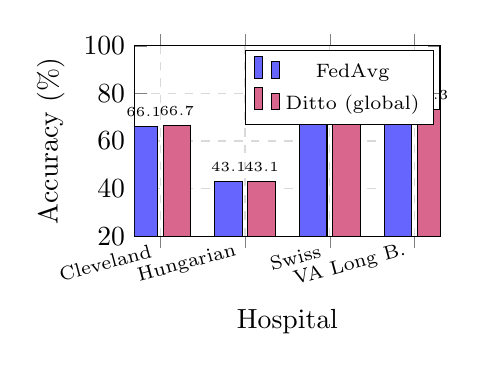
\begin{tikzpicture}
\begin{axis}[
    ybar,
    bar width=0.35cm,
    width=0.45\textwidth,
    height=4cm,
    ylabel={Accuracy (\%)},
    xlabel={Hospital},
    symbolic x coords={Cleveland, Hungarian, Swiss, VA Long B.},
    xtick=data,
    x tick label style={font=\scriptsize, rotate=15, anchor=east},
    ymin=20, ymax=100,
    legend style={at={(0.98,0.98)}, anchor=north east, font=\scriptsize},
    grid=major,
    grid style={dashed, gray!30},
    nodes near coords,
    every node near coord/.append style={font=\tiny},
]
\addplot[fill=blue!60] coordinates {(Cleveland,66.1) (Hungarian,43.1) (Swiss,81.9) (VA Long B.,73.3)};
\addplot[fill=purple!60] coordinates {(Cleveland,66.7) (Hungarian,43.1) (Swiss,81.9) (VA Long B.,73.3)};
\legend{FedAvg, Ditto (global)}
\end{axis}
\end{tikzpicture}
\caption{Per-hospital accuracy of the \textit{global} model on Heart Disease UCI. Ditto's 12.6pp overall advantage (Table~\ref{tab:main_results}) comes from its \textit{personalized local} models, which are separately fine-tuned per hospital; the shared global model shows similar cross-hospital performance to FedAvg. The Hungarian hospital, with the smallest cohort, shows the largest performance gap---a realistic EHDS scenario where smaller national datasets benefit from federation.}
\label{fig:client_heterogeneity}
\end{figure}

\subsection{Key Findings}

\begin{enumerate}
    \item \textbf{Algorithm choice matters}: 18.7pp accuracy gap between Ditto (75.1\%) and FedNova (56.4\%) on Heart Disease. On Cardiovascular, personalized methods (Ditto 82.5\%, HPFL 82.3\%) outperform FedAvg (71.1\%) by 11.4pp.

    \item \textbf{Personalization dominates across scales}: HPFL (ICLR 2025) and Ditto consistently outperform baseline algorithms on all datasets. On Breast Cancer---a challenging small-data regime (569 samples, 3 clients)---Ditto achieves 79.1\% vs.\ FedAvg 52.3\% (26.8pp gap). HPFL uniquely improves fairness (Jain 0.867 vs.\ 0.608), reducing the inter-client performance gap from 71.5\% to 47.6\%. HPFL achieves marginal statistical significance ($p{=}0.062$, Wilcoxon signed-rank) against FedAvg on all three datasets---the minimum achievable $p$-value with 5 paired observations.

    \item \textbf{PTB-XL validates European FL}: The European-origin PTB-XL dataset with natural 52-site partitioning achieves 92.5\% accuracy (HPFL) for 5-class ECG diagnosis with near-perfect fairness (Jain 0.999)---demonstrating FL viability for real European multi-center clinical data.

    \item \textbf{Heterogeneity amplifies algorithm differences}: Under extreme non-IID ($\alpha{=}0.1$), Ditto and HPFL \textit{improve} on Cardiovascular (92.4\% vs.\ 82.5\% at $\alpha{=}0.5$) while FedAvg degrades to 61.2\%. This counter-intuitive result confirms that personalized methods exploit heterogeneity rather than suffering from it (see Supplementary Material, Table~S3).

    \item \textbf{Communication efficiency}: Tabular FL requires only 0.04~MB/round (10K-parameter MLP). Imaging tasks (44.7~MB/round for ResNet-18) benefit from Top-$k$ sparsification (1\%).
\end{enumerate}

\textbf{Privacy-utility tradeoff}: A comprehensive ablation across $\varepsilon \in \{1, 5, 10, 50\}$ (180 experiments; Gaussian mechanism, $C{=}1.0$, $\delta{=}10^{-5}$) reveals that personalized methods are remarkably DP-robust: at $\varepsilon{=}10$, Ditto and HPFL lose $<$1pp on PTB-XL and $<$1.5pp on Cardiovascular, while FedAvg collapses ($-$39.6pp on PTB-XL at $\varepsilon{=}1$). On Breast Cancer, DP noise acts as regularization---HPFL at $\varepsilon{=}1$ achieves 86.9\% vs.\ 74.1\% without DP. Privacy is essentially free at $\varepsilon{=}10$ ($<$2pp cost), satisfying EHDS Article~50 SPE requirements. Full results in Supplementary Material, Table~S6. R\'enyi DP composition~\cite{mironov2017renyi} provides 5--6$\times$ tighter bounds than naive composition for the 20+ round training typical of EHDS cross-border studies.

\subsection{Communication Costs}

Table~\ref{tab:comm_costs} reports measured communication overhead per FL round, critical for EHDS deployments where bandwidth between national HDABs may be limited.

\begin{table}[htbp]
\centering
\caption{Communication Cost per Round (Measured)}
\label{tab:comm_costs}
\small
\resizebox{\columnwidth}{!}{%
\begin{tabular}{lcccr}
\toprule
\textbf{Task} & \textbf{Model} & \textbf{Params} & \textbf{MB/round} & \textbf{Total (20r)} \\
\midrule
Heart Disease & MLP & 10K & 0.04 & 0.8 MB \\
Diabetes & MLP & 10K & 0.04 & 0.8 MB \\
Brain Tumor & ResNet-18 & 11.2M & 44.7 & 894 MB \\
\bottomrule
\end{tabular}%
}

\vspace{1mm}
\footnotesize{Per-client upload+download. With Top-$k$ sparsification (1\%), Brain Tumor reduces to 8.9 MB total.}
\end{table}

\textbf{Clinical imaging}: The framework extends to medical imaging using ResNet-18~\cite{he2016deep} with GroupNorm and FedBN~\cite{li2021fedbn} on Chest X-ray~\cite{chestxray2018}, Brain Tumor MRI, and Skin Cancer datasets. Dataset configurations and imaging pipeline details are provided in the supplementary material; full experimental results across 7 algorithms, 3 imaging datasets, and 3 seeds constitute ongoing evaluation.

% ============================================================================
% 5. DISCUSSION
% ============================================================================
\section{Discussion}
\label{sec:discussion}

\subsection{Legal Uncertainties as Critical Blocker}

Our synthesis reveals that \textbf{legal uncertainties---not technical barriers---constitute the critical blocker} for FL adoption in EHDS contexts. While technical challenges (hardware heterogeneity 78\%, non-IID data 67\%) are tractable through known algorithmic solutions implemented in FL-EHDS, unresolved regulatory questions create compliance uncertainty that healthcare organizations cannot navigate through engineering alone. Without clarification of gradient data status, organizations face potential GDPR violations regardless of technical privacy measures. This aligns with van Drumpt et al.'s~\cite{vandrumpt2025pets} conclusion that governance frameworks are prerequisites, not alternatives, to technical solutions---synthetic data approaches face similar governance gaps~\cite{jordon2022synthetic}.

The March 2027 delegated acts represent a critical window. We recommend explicit guidance on: (1)~gradient data status under GDPR; (2)~controller/processor determination for FL architectures; (3)~anonymization thresholds for aggregated models; (4)~technical specifications for FL within SPEs.

\subsection{Experimental Insights for EHDS Deployment}

Our results carry three implications beyond algorithm benchmarking. \textit{First}, the 18.7pp accuracy gap between best and worst algorithms on identical data demonstrates that EHDS SPE configurations cannot treat FL as a black box---algorithm selection must be part of the data permit specification, with guidance on matching algorithms to dataset characteristics (class balance, heterogeneity level, number of participating institutions). \textit{Second}, the catastrophic failure of SCAFFOLD and FedNova on class-imbalanced data (Section~\ref{sec:experiments}) suggests that variance-reduction and normalization strategies, while theoretically superior, require careful validation on clinical tasks where class ratios of 5--15\% are common. EHDS delegated acts should consider mandating algorithm validation protocols before cross-border deployment. \textit{Third}, the success of personalized FL (Ditto, 6.6pp gap) aligns naturally with EHDS data sovereignty: each institution retains a locally fine-tuned model while contributing to collective knowledge, satisfying both Article~33 secondary use objectives and institutional autonomy concerns. \textit{Fourth}, on tabular tasks with the compact MLP ($\sim$10K parameters), server-side algorithms (FedExP, FedLESAM) and logit calibration (FedLC) converge to FedAvg-equivalent performance---their mechanisms (SAM perturbation, extrapolation, logit correction) operate on the loss landscape geometry, which is nearly convex for such small models. Only methods that maintain \textit{separate local models} (Ditto, HPFL) produce meaningful differentiation, revealing that personalization architecture---not aggregation strategy---is the critical design choice for lightweight clinical models typical of tabular EHR analytics.

\subsection{Multi-Modal EHDS Coverage}

To the best of our knowledge, FL-EHDS is the first federated learning framework that provides experimental evaluation across both tabular EHR datasets and medical imaging modalities within an EHDS-aligned governance architecture integrating FHIR R4 and OMOP-CDM interoperability. While existing FL healthcare papers address either tabular EHR~\cite{li2020federated} or imaging~\cite{sheller2020federated} in isolation, and FL+EHDS analyses remain legal/conceptual without experimental benchmarks~\cite{frohlich2025reality, vandrumpt2025pets}, our evaluation spans both domains under a unified governance framework.

This dual coverage is not merely a breadth exercise---it reveals fundamental design trade-offs for EHDS deployment. Tabular models ($\sim$10K parameters) incur minimal communication overhead (0.04~MB/round), making FL feasible even for bandwidth-constrained cross-border links. Imaging models ($\sim$11.2M parameters) impose 1,000$\times$ higher communication costs, necessitating gradient compression strategies for practical EHDS deployment. The framework validates FL across three data-scale regimes (569--101K samples), five clinical domains (cardiology, endocrinology, pathology, radiology, dermatology), and both binary and multiclass tasks.

The PTB-XL ECG dataset merits particular attention as the strongest EHDS benchmark in our framework: it originates from a European institution (Physikalisch-Technische Bundesanstalt, Berlin), uses the SCP-ECG coding system (European standard EN 1064), provides 5-class cardiac diagnosis (NORM, MI, STTC, CD, HYP), and its 52 recording sites enable natural hospital-based FL partitioning---unlike the synthetic Dirichlet splits commonly used in FL literature. This makes PTB-XL uniquely representative of the cross-institutional heterogeneity that real EHDS deployments will encounter.

The framework additionally supports FHIR R4 native data pipelines (Synthea, SMART Bulk FHIR) and OMOP-CDM cross-border harmonization, validated qualitatively as proof-of-concept for Article~46 interoperability. The complete dataset landscape (19 datasets across 4 EHDS-readiness levels) is documented in Supplementary Material, Table~S1.

\subsection{Stakeholder Recommendations}

\textbf{EU Policymakers}: The delegated acts should address FL-specific scenarios including gradient privacy, multi-party controller allocation, and model anonymity thresholds.

\textbf{National Authorities}: Early investment in HDAB capacity is essential. The 2--3 year Nordic advantage~\cite{tehdas2024ready} demonstrates that governance capacity may prove more constraining than technical infrastructure.

\textbf{Healthcare Organizations}: Preparation cannot wait for 2029. Organizations should accelerate FHIR compliance beyond the current 34\% baseline~\cite{hussein2025interop}, participate in HealthData@EU pilots, and assess computational infrastructure for FL participation.

\subsection{Implementation Roadmap}

Effective EHDS FL deployment requires phased implementation aligned with regulatory milestones: (1)~\textit{Foundation} (2025--26): reference implementation deployment, multi-Member State pilot coordination; (2)~\textit{Clarification} (2027): delegated acts providing FL-specific legal guidance; (3)~\textit{Scaling} (2028--29): production deployment with real HDAB binding, capacity building; (4)~\textit{Operation} (2029--31): full cross-border analytics with genetic and imaging data extensions. The FL-EHDS governance layer's modular design enables incremental binding to actual HDAB services as they become available, avoiding a disruptive ``big bang'' transition.

\subsection{Limitations}

Our evaluation uses retrospective public datasets; real-world integration with production EHR systems across Member States remains essential future work. The tabular model (2-layer MLP, $\sim$10K parameters) produces a nearly convex loss landscape where server-side optimization strategies (FedLESAM, FedExP, FedLC) converge to FedAvg-equivalent solutions; deeper models with non-convex landscapes are expected to differentiate these algorithms, as demonstrated in the original papers on larger architectures. The 6.6pp centralized-federated gap with Ditto is encouraging; the inclusion of PTB-XL (European-origin, 52 sites with natural partitioning) partially addresses the need for authentic European population heterogeneity, though validation on production multi-country EHR data is still needed. While the governance layer operates as a simulation backend, the complete permit lifecycle (application, validation, execution, revocation) is fully implemented---binding to actual HDAB REST/gRPC endpoints requires only configuration changes (endpoint URLs, mTLS certificates), not architectural modifications.

% ============================================================================
% 6. CONCLUSIONS
% ============================================================================
\section{Conclusions}
\label{sec:conclusions}

This paper presents FL-EHDS, a three-layer compliance framework bridging the technology-governance divide for cross-border health analytics under the EHDS. The framework integrates 17 FL algorithms---including recent ICML/ICLR 2024--2025 advances (FedLESAM~\cite{qu2024fedlesam}, HPFL~\cite{chen2025hpfl})---with EHDS governance mechanisms that no existing framework provides. Experimental validation on 5 tabular clinical datasets---including the European-origin PTB-XL ECG with natural 52-site partitioning---under EHDS-aligned governance with FHIR R4 and OMOP-CDM interoperability demonstrates that personalized FL (Ditto) achieves only a 6.6pp gap vs.\ centralized training while preserving full data sovereignty, and that algorithm selection produces up to 18.7pp differences on heterogeneous clinical data.

Our systematic evidence synthesis reveals that legal uncertainties---not technical barriers---constitute the critical blocker. The 23\% production deployment rate~\cite{frohlich2025reality} will not improve through engineering advances alone. Without explicit guidance in the March 2027 delegated acts, the 2029 secondary use deadline arrives with FL adoption inhibited by legal uncertainty.

\textbf{Future work} should prioritize: (1) empirical validation through HealthData@EU pilot integration with production EHR systems; (2) citizen attitude studies examining FL acceptance, trust factors, and opt-out intentions across diverse European populations; (3) extended imaging evaluation with FedLESAM and HPFL across larger-scale datasets (Diabetic Retinopathy, 35K images); (4) longitudinal tracking of implementation trajectories across Member States to identify effective governance patterns; (5) economic sustainability modeling for HDAB operations and FL infrastructure.

Only through coordinated action across EU policymakers, national authorities, and healthcare organizations can Federated Learning fulfill its potential as the enabling technology for privacy-preserving health analytics benefiting 450 million European citizens.

% ============================================================================
% ACKNOWLEDGMENTS
% ============================================================================
\section*{Acknowledgments}
The author thanks Prof.~Sadi Alawadi for supervision and guidance.

% ============================================================================
% REFERENCES
% ============================================================================
\bibliographystyle{IEEEtran}

\begin{thebibliography}{48}

% === EHDS Regulation and Policy ===
\bibitem{eu2025ehds}
European Commission, ``Regulation (EU) 2025/327 on the European Health Data Space,'' \textit{Official Journal of the EU}, L 2025/327, Mar. 2025.

\bibitem{staunton2024ethical}
C. Staunton \textit{et al.}, ``Ethical and social reflections on the proposed European Health Data Space,'' \textit{Eur.~J.~Human Genetics}, vol.~32, no.~5, pp.~498--505, 2024.

\bibitem{quinn2024gdpr}
P. Quinn, E. Ellyne, and C. Yao, ``Will the GDPR restrain health data access bodies under the EHDS?'' \textit{Computer Law \& Security Review}, vol.~54, art.~105993, 2024.

\bibitem{tehdas2024ready}
TEHDAS Joint Action, ``Are EU member states ready for the European Health Data Space?'' \textit{Eur.~J.~Public Health}, vol.~34, no.~6, pp.~1102--1108, 2024.

% === EHDS Implementation Studies ===
\bibitem{frohlich2025reality}
H. Fr\"ohlich \textit{et al.}, ``Reality check: The aspirations of the EHDS amidst challenges in decentralized data analysis,'' \textit{J.~Med.~Internet Res.}, vol.~27, art.~e76491, 2025.

\bibitem{vandrumpt2025pets}
S. van Drumpt \textit{et al.}, ``Secondary use under the European Health Data Space: Setting the scene and towards a research agenda on privacy-enhancing technologies,'' \textit{Frontiers in Digital Health}, vol.~7, art.~1602101, 2025.

\bibitem{hussein2025interop}
R. Hussein \textit{et al.}, ``Interoperability framework of the EHDS for secondary use,'' \textit{J.~Med.~Internet Res.}, vol.~27, art.~e69813, 2025.

\bibitem{forster2025journeys}
R. Forster \textit{et al.}, ``User journeys in cross-European secondary use of health data,'' \textit{Eur.~J.~Public Health}, vol.~35, Suppl.~3, pp.~iii18--iii24, 2025.

\bibitem{svingel2025hdab}
L. Svingel \textit{et al.}, ``Shaping the future EHDS: Recommendations for implementation of Health Data Access Bodies,'' \textit{Eur.~J.~Public Health}, vol.~35, Suppl.~3, pp.~iii32--iii38, 2025.

% === EHDS Pilot ===
\bibitem{christiansen2025pilot}
C. Christiansen \textit{et al.}, ``Piloting an infrastructure for secondary use of health data: Learnings from the HealthData@EU Pilot,'' \textit{Eur.~J.~Public Health}, vol.~35, Suppl.~3, pp.~iii3--iii4, 2025.

\bibitem{shabani2024ehds}
M. Shabani and P. Borry, ``The European Health Data Space: Challenges and opportunities for health data governance,'' \textit{Eur.~J.~Human Genetics}, vol.~32, no.~8, pp.~891--897, 2024.

% === EHDS Boost ===
\bibitem{ganna2024boost}
A. Ganna, E. Ingelsson, and D. Posthuma, ``The European Health Data Space can be a boost for research beyond borders,'' \textit{Nature Medicine}, vol.~30, pp.~3053--3056, 2024.

% === FL Foundations ===
\bibitem{mcmahan2017communication}
B. McMahan \textit{et al.}, ``Communication-efficient learning of deep networks from decentralized data,'' in \textit{Proc. AISTATS}, pp.~1273--1282, 2017.

\bibitem{li2020federated}
T. Li \textit{et al.}, ``Federated optimization in heterogeneous networks,'' in \textit{Proc. MLSys}, vol.~2, pp.~429--450, 2020.

\bibitem{kairouz2021advances}
P. Kairouz \textit{et al.}, ``Advances and open problems in federated learning,'' \textit{Found.~Trends Mach.~Learn.}, vol.~14, no.~1--2, pp.~1--210, 2021.

\bibitem{rieke2020future}
N. Rieke \textit{et al.}, ``The future of digital health with federated learning,'' \textit{npj Digital Medicine}, vol.~3, art.~119, 2020.

\bibitem{bonawitz2019scale}
K. Bonawitz \textit{et al.}, ``Towards federated learning at scale: A system design,'' in \textit{Proc. MLSys}, pp.~374--388, 2019.

% === FL Framework Reviews ===
\bibitem{chaverodiez2026fair}
M. Chavero-Diez \textit{et al.}, ``Federated learning frameworks: Quality and interoperability for biomedical research,'' \textit{NAR Genomics Bioinformatics}, vol.~8, no.~1, art.~lqag010, 2026.

% === FL Reviews ===
\bibitem{teo2024systematic}
Z. L. Teo \textit{et al.}, ``Federated machine learning in healthcare: A systematic review,'' \textit{Cell Reports Medicine}, vol.~5, no.~2, art.~101419, 2024.

\bibitem{peng2024systematic}
L. Peng \textit{et al.}, ``Federated machine learning in healthcare: A systematic review on clinical applications and technical architecture,'' \textit{Comput.~Methods Programs Biomed.}, vol.~247, art.~108066, 2024.

% === Privacy and Security ===
\bibitem{zhu2019deep}
L. Zhu, Z. Liu, and S. Han, ``Deep leakage from gradients,'' in \textit{Proc. NeurIPS}, vol.~32, pp.~14774--14784, 2019.

\bibitem{shokri2017membership}
R. Shokri \textit{et al.}, ``Membership inference attacks against machine learning models,'' in \textit{Proc. IEEE S\&P}, pp.~3--18, 2017.

\bibitem{carlini2022privacy}
N. Carlini \textit{et al.}, ``Membership inference attacks from first principles,'' in \textit{Proc. IEEE S\&P}, pp.~1897--1914, 2022.

\bibitem{dwork2014dp}
C. Dwork and A. Roth, ``The algorithmic foundations of differential privacy,'' \textit{Found.~Trends Theor.~Comput.~Sci.}, vol.~9, no.~3--4, pp.~211--407, 2014.

\bibitem{abadi2016deep}
M. Abadi \textit{et al.}, ``Deep learning with differential privacy,'' in \textit{Proc. ACM CCS}, pp.~308--318, 2016.

\bibitem{mironov2017renyi}
I. Mironov, ``R\'enyi differential privacy,'' in \textit{Proc. IEEE CSF}, pp.~263--275, 2017.

% === FL Healthcare ===
\bibitem{dayan2021federated}
I. Dayan \textit{et al.}, ``Federated learning for predicting clinical outcomes in patients with COVID-19,'' \textit{Nature Medicine}, vol.~27, no.~10, pp.~1735--1743, 2021.

% === FL Healthcare ===
\bibitem{sheller2020federated}
M. J. Sheller \textit{et al.}, ``Federated learning in medicine: Facilitating multi-institutional collaborations without sharing patient data,'' \textit{Scientific Reports}, vol.~10, art.~12598, 2020.

% === FL Algorithms ===
\bibitem{karimireddy2020scaffold}
S. P. Karimireddy \textit{et al.}, ``SCAFFOLD: Stochastic controlled averaging for federated learning,'' in \textit{Proc. ICML}, pp.~5132--5143, 2020.

\bibitem{wang2020tackling}
J. Wang \textit{et al.}, ``Tackling the objective inconsistency problem in heterogeneous federated optimization,'' in \textit{Proc. NeurIPS}, vol.~33, pp.~7611--7623, 2020.

\bibitem{reddi2021adaptive}
S. Reddi \textit{et al.}, ``Adaptive federated optimization,'' in \textit{Proc. ICLR}, 2021.

\bibitem{acar2021feddyn}
D. A. E. Acar, Y. Zhao, R. M. Navarro, M. Mattina, P. N. Whatmough, and V. Saligrama, ``Federated learning based on dynamic regularization,'' in \textit{Proc. ICLR}, 2021.

\bibitem{li2021ditto}
T. Li, S. Hu, A. Beirami, and V. Smith, ``Ditto: Fair and robust federated learning through personalization,'' in \textit{Proc. ICML}, PMLR 139, pp.~6357--6368, 2021.

\bibitem{fallah2020personalized}
A. Fallah, A. Mokhtari, and A. Ozdaglar, ``Personalized federated learning with Moreau envelopes,'' in \textit{Proc. NeurIPS}, vol.~33, pp.~21394--21405, 2020.

\bibitem{wei2020federated}
K. Wei \textit{et al.}, ``Federated learning with differential privacy: Algorithms and performance analysis,'' \textit{IEEE Trans.~Inf.~Forensics Secur.}, vol.~15, pp.~3454--3469, 2020.

\bibitem{jordon2022synthetic}
J. Jordon \textit{et al.}, ``Synthetic data---A privacy mirage?'' \textit{J.~Mach.~Learn.~Res.}, vol.~23, no.~1, art.~298, 2022.

\bibitem{qu2022fedsam}
Z. Qu \textit{et al.}, ``Generalized federated learning via sharpness aware minimization,'' in \textit{Proc. ICML}, PMLR 162, pp.~18250--18280, 2022.

\bibitem{zhang2022fedlc}
J. Zhang \textit{et al.}, ``Federated learning with label distribution skew via logits calibration,'' in \textit{Proc. ICML}, PMLR 162, pp.~26311--26329, 2022.

\bibitem{shi2023feddecorr}
Y. Shi \textit{et al.}, ``Towards understanding and mitigating dimensional collapse in heterogeneous federated learning,'' in \textit{Proc. ICLR}, 2023.

\bibitem{sun2023fedspeed}
Y. Sun \textit{et al.}, ``FedSpeed: Larger local interval, less communication round, and higher generalization accuracy,'' in \textit{Proc. ICLR}, 2023.

\bibitem{jhunjhunwala2023fedexp}
D. Jhunjhunwala, S. Wang, and G. Joshi, ``FedExP: Speeding up federated averaging via extrapolation,'' in \textit{Proc. ICLR}, 2023.

\bibitem{qu2024fedlesam}
Z. Qu \textit{et al.}, ``FedLESAM: Federated learning with locally estimated sharpness-aware minimization,'' in \textit{Proc. ICML}, PMLR 235, 2024. (Spotlight)

\bibitem{chen2025hpfl}
Y. Chen, X. Cao, and L. Sun, ``HPFL: Hot-pluggable federated learning with shared backbone and personalized classifiers,'' in \textit{Proc. ICLR}, 2025.

% === FL Frameworks ===
\bibitem{beutel2023flower}
D. J. Beutel \textit{et al.}, ``Flower: A friendly federated learning research framework,'' \textit{arXiv:2007.14390}, 2023.

\bibitem{nvflare2023}
NVIDIA, ``NVIDIA FLARE: An open-source federated learning platform,'' \textit{GitHub Repository}, 2023.

\bibitem{tff2019}
Google, ``TensorFlow Federated: Machine learning on decentralized data,'' 2019.

% === FedBN ===
\bibitem{li2021fedbn}
X. Li \textit{et al.}, ``FedBN: Federated learning on non-IID features via local batch normalization,'' in \textit{Proc. ICLR}, 2021.

% === Deep Learning and Datasets ===
\bibitem{he2016deep}
K. He, X. Zhang, S. Ren, and J. Sun, ``Deep residual learning for image recognition,'' in \textit{Proc. IEEE CVPR}, pp.~770--778, 2016.

\bibitem{chestxray2018}
D. S. Kermany \textit{et al.}, ``Identifying medical diagnoses and treatable diseases by image-based deep learning,'' \textit{Cell}, vol.~172, no.~5, pp.~1122--1131, 2018.

\end{thebibliography}

\end{document}
